% Small introtext to motivate this chapter. What am I going to go over here.

% The friction force is not an independent external force that acts on a body but an internal force that opposes the externally applied force. Thus, it may be thought of as a reaction force rather than an action force. In this sense, it is similar to the adhesion force between two bodies, which appears only when one tries to separate the bodies from contact. \cite{gao_frictional_2004}





\chapter{Friction} % Tribology - fiction
Friction plays a central role for the topic of this thesis, as this is the key concept that we want to explore through design of microstructures. In this chapter we review relevant theoretical understanding and highlight the theoretical expectations for our study.
\\

Friction is a part of the wider field tribology which includes the study of
friction, wear and lubrication between two surfaces in relative motion \cite[p.
1]{gnecco_meyer_2015}. In this thesis we will only concern ourselves with so-called wearless dry friction. That is, without any use of lubrication and without any resulting wear of the contacting surfaces. 

\section{Friction across scales}
Tribological systems take place across a broad
range of time and length scales, ranging from geological stratum layers involved
in earthquakes \cite{kim_nano-scale_2009} to microscopic atomistic processes, as
in the gliding motion of a nanocluster of a nanomotor \cite{Manini_2016}. This
vast difference in scale gives rises to different frictional mechanism being
dominating at different scales. On a macro scale the system is usally subject
to relatively high load and sliding speed leading to high contact stress and
wear. On the other hand, the micro-/nanoscale regime occupies the opposite domain operating under relatviely small load and sliding speed with negligible wear \cite{kim_nano-scale_2009} \cite[p. 5]{bhushan_2013}. While macroscale friction is often reduced into a few variables such as load, material type, sliding speed and surface roughness it is clear that the micro-/nanoscale friction cannot be generalized under such a simple representation. On the micro-/nanoscale the tribological propteries are dominated by surface properties which will introduce an additional sensitivity to variables such as temperature, humidity and even sliding history. The works of Bhushan and Kulkarni \cite[(1996)]{BHUSHAN199649} showed that the friction coefficient decreased with scale even though the materials used was unchanged. This reveals an intrinsic relationship between friction and scale as the contact condition is altered.

The phenomenological descriptions of macroscale friction cannot yet be derived from the fundamental atomic principles, and bridging the gap between different length scales in tribological systems remains an open challenge \cite{Manini_2016}. Hence, the following sections will be organized into macro-, micro- and nanoscale representing the theoretical understanding governing each scale regime. While our study of the graphene sheet is based on a nanoscale perspective the hypothesizing about application possibilities will eventually draw upon a macroscale perspective as well. Thus, we argue that a brief theoretical introduction to all three major scales is suitable for a more complete interpreation of the findings in this thesis. 


% Tribological systems pose a wide range of dimensional scale. At the largest
% scale, geological stratum layers that are involved in earthquakes may be
% considered as a tribological system. The movement of the stratum occurs when
% the frictional forces between the layers are overcome by internal pressure
% inside the earth. At the smallest scale, relative motion of atoms at the
% interface of two materials would be a good example that involves frictional
% interaction. Owing to the vast difference in scale, the dominant mechanisms of
% friction and wear in macro-scale systems may be different from those of
% micro/nano-scale systems. In macro-scale, the tribological systems experience
% relatively large contact stresses and speeds. On the other hand,
% micro/nano-scale systems operate under relatively low loads and speeds.
% Particularly, the inertial effects that are prominent in macro-scale may be
% insignificant at the micro/nano-scale. Rather, surface forces often dictate
% the tribological interactions at small scales. \cite{kim_nano-scale_2009}.




% The differences between the conventional or macrotribology and
% micro/nanotribology are contrasted in Figure 1.3.1. In macrotribology, tests
% are conducted on components with relatively large mass under heavily loaded
% conditions. In these tests, wear is inevitable and the bulk prop- erties of
% mating components dominate the tribological performance. In
% micro/nanotribology, measurements are made on components, at least one of the
% mating components, with relatively small mass under lightly loaded conditions.
% In this situation, negligible wear occurs and the surface properties dominate
% the tribological performance. \cite{bhushan_2013}[p. 5]



% Quotes: Sliding friction that takes place between two surfaces in the absence
% of lubricant is termed "dry" friction even if the process occurs in an ambient
% environment. (Nanotribology and Nanomechanics, p. 329)




% We were astonished to discover that molecules that could flex or slide even
% just a little in response to the oscillatory motion of the microbalance were
% linked to low friction levels at the macro-scale. Put another way,
% exceptionally low friction at the atomic scale was not a prerequisite for the
% substantial reduction in macroscopic friction.
% (\url{https://physicsworld.com/a/friction-at-the-nano-scale/})



% Sliding friction that takes place between two surfaces in the absence of
% lubricant is termed ``dry''  friction even if the process occurs in an ambient
% environment. (Nanotriology and Nanomechanics, p. 329)



% It is generally accepted that friction is caused by more than one mechanism in
% a given sliding system. Generally, frictional force arises due to two
% fundamentally different causes, namely one that is mechanical in nature and
% the other being chemical in its origin. In the case of mechanical cause of
% friction, plowing of the surface by hard particles or asperities is mainly
% responsible for generating the frictional force.2,4,5-7 As for the chemical
% mechanism of friction, adhesion between surfaces of the two solids in contact
% is the cause of friction.2,4,5,8 Another point to note is that tribological
% phenomena are heavily dependent on system parameters of the operating machine
% such as speed, temperature, load, and environment. As such, the dominating.
% \cite{kim_nano-scale_2009}.







\section{Macroscale}
Our working definition of the \textit{macroscale} is everything on the scale of visible objects. This is usually denoted to the size of milimeters \SI{e-3}{\metre} and above. Most importantly, we want to make a distinction to the microscale, where the prefix indicates the size of micrometers $m^{-6}$. Hence, we essentially consider everything larger than \textit{micro} to belong to the macroscale\footnote{The width of a human hair is often used as a reference for the limit of human perception. Since the width of a human hair is on the length scale $10^{-5}$ to \SI{e-4}{m} we find that this definition of the lower perceptional limit alligns rather well with the transistion from macro- to microscale.}.

\subsection{Amontons’ law}
% Based on \cite{gnecco_meyer_2015}
% and \cite{gao_frictional_2004}
 
 In order to start and keep a solid block moving against a solid surface we must
 overcome certain frictional forces $F_{\text{fric}}$ \cite{gnecco_meyer_2015}.
 The static friction force $F_s$ corresponds to the minimum tangential force
 required to initiate the sliding while the kintec friciton force $F_k$
 corresponds to the tangential force needed to sustain such a sliding at steady
 speed. The work of Leonardo da Vinci (1452–1519), Guillaume Amontons (1663-705)
 and Charles de Coulomb (1736-1806) all contributed to the empirical law,
 commonly known as \textit{Amontons’ law}, which serves as a common base for macroscale
 friction. Amontons’ law states that the fricitonal forces is entirely
 independent of contact area and sliding velocity. Instead, it relies only on
 the normal force $F_N$, acting perpendicular to the surface, and the material specific friction coefficient $\mu$ as
\begin{align}
  F_{\text{fric}} = \mu F_N.
  \label{eq:amonton}
\end{align}
Notice that the term \textit{Normal force} is often used interchangeably
with \textit{load} and \textit{normal load} allthough the latter two terms refer to the applied force, ``pushing'' the object into the surface, and the first is the reaction force acting from the surface on the object. In equilibrium, these forces are equal in magnitude and hence we will not make a distinction between these terms. On the same note, the frictional force is different from a conventional force which in the Newtonian definition acts on a body from the outside and make it accelerate \cite{gao_frictional_2004}. Rather than being an independent external force the friction force is an internal \textit{reaction} force opposing the externally applied ``sliding'' force. 

The friction coeffcient $\mu$ is typically different for the cases of static
($\mu_s$) and kinetic ($\mu_k$) friction, usually both with values lower than
one and $\mu_s \ge \mu_k$ in all cases \cite[p. 6]{gnecco_meyer_2015}. The
friction coefficient is taken to be a constant defined by either
\cite{gao_frictional_2004} \\
\vspace{0.1cm}
\begin{subequations}
\noindent\begin{minipage}{.2\linewidth}
  \hfill
\end{minipage}
\begin{minipage}[b]{0.2\linewidth}
  \begin{align}
    \mu_1 = \frac{F_{\text{fric}}}{F_N},
    \label{eq:mu_def1}
  \end{align}
\end{minipage}
\begin{minipage}[b]{0.2\linewidth}
  \begin{align*}
    \text{or}
  \end{align*}
\end{minipage}
\begin{minipage}[b]{0.2\linewidth}
  \begin{align}
    \mu_2 = \frac{dF_{\text{fric}}}{dF_N}.
    \label{eq:mu_def2}
  \end{align}
\end{minipage}
\begin{minipage}{.2\linewidth}
\end{minipage}
\label{eq:mu_def}
\end{subequations}
\vspace{0.1cm}
\\
\noindent The first definition \cref{eq:mu_def1} requires zero friction at zero
load, i.e.\ $F_{\text{fric}} = 0$ at $F_N = 0$, while the second definition
(\cref{eq:mu_def2}) allows for a finite friction force at zero load since the
coefficient is instead given by the slope of the $F_{\text{fric}}$ vs.\ $F_N$
curve. The consequences of the two different definitions are illustrated in
\cref{fig:fric_coef_example}. Usually the friction force is not zero under
zero load (red curve: Linear + shift) due to adhesive forces \hl{source}, which
constitutes an additional constant added to Amontons’ law in \cref{eq:amonton}. Using the first definition (\cref{eq:mu_def1}) would make the friction coefficient diverge for low load as illustrated in \cref{fig:fric_coef_example}, and thus we will use the second definition (\cref{eq:mu_def2}) moving forward. This also allows for a better interpretation in cases where Amontons’ law does not hold true and the friction force change non-linear with load (Purple curve in \cref{fig:fric_coef_example}).

% In reality the friction coeffcient is not truly a material specific constant as it is often found to vary under different conditions such as humidity or smooth and rough morphologies of the sliding surfaces \cite{gao_frictional_2004}. 


\begin{figure}[H]
  \centering
  \begin{subfigure}[t]{0.32\textwidth}
      \centering
      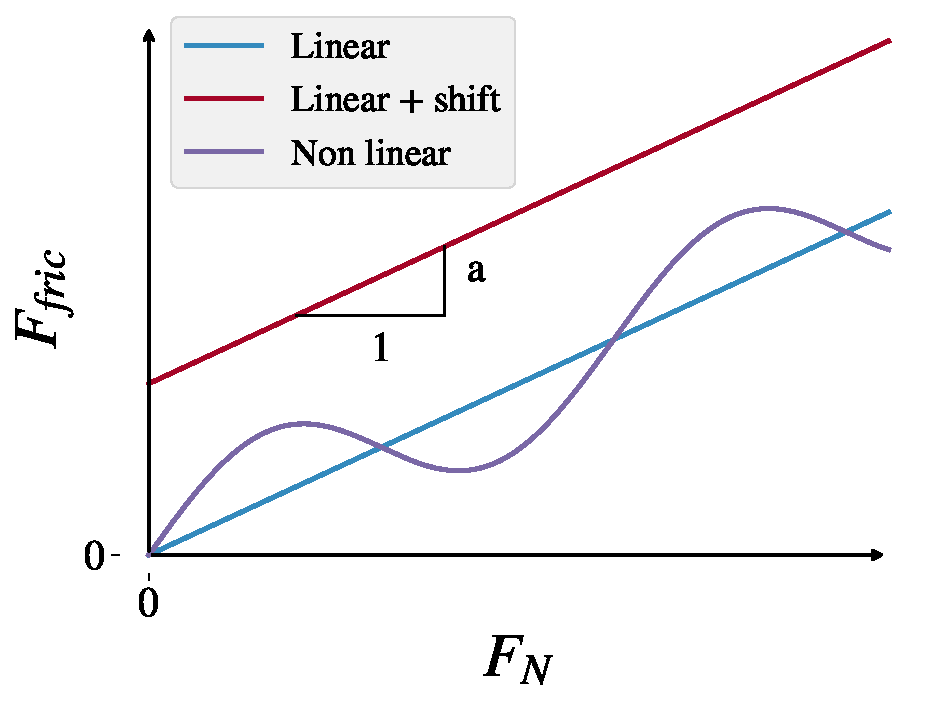
\includegraphics[width=\textwidth]{figures/theory/fric_coef_example_a.pdf}
      \caption{}
      % \label{fig:}
  \end{subfigure}
  \hfill
  \begin{subfigure}[t]{0.32\textwidth}
      \centering
      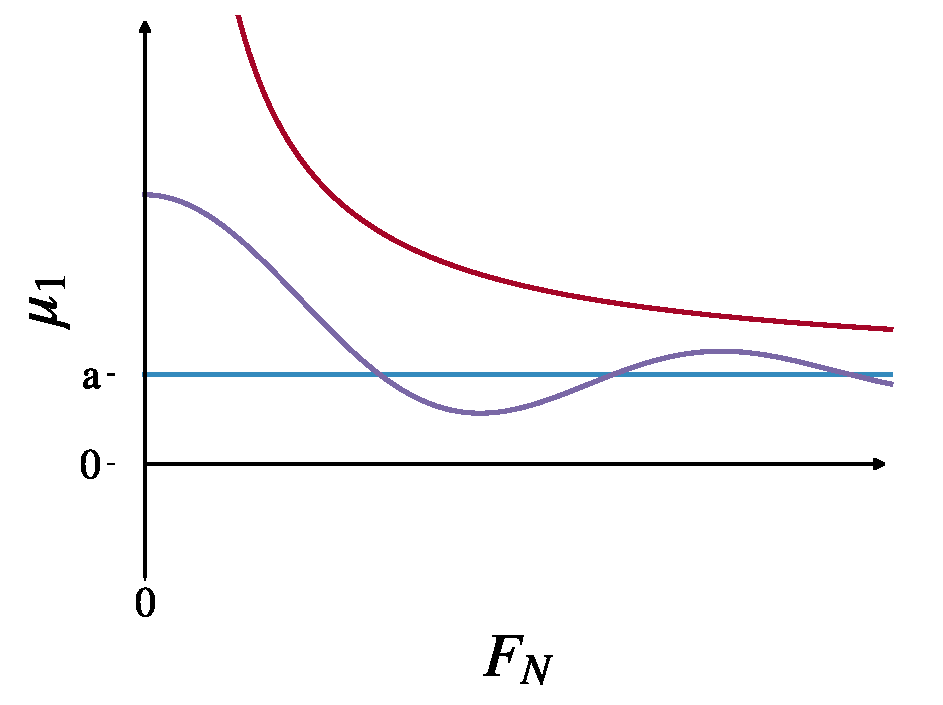
\includegraphics[width=\textwidth]{figures/theory/fric_coef_example_b.pdf}
      \caption{}
      % \label{fig:}
  \end{subfigure}
  \hfill
  \begin{subfigure}[t]{0.32\textwidth}
      \centering
      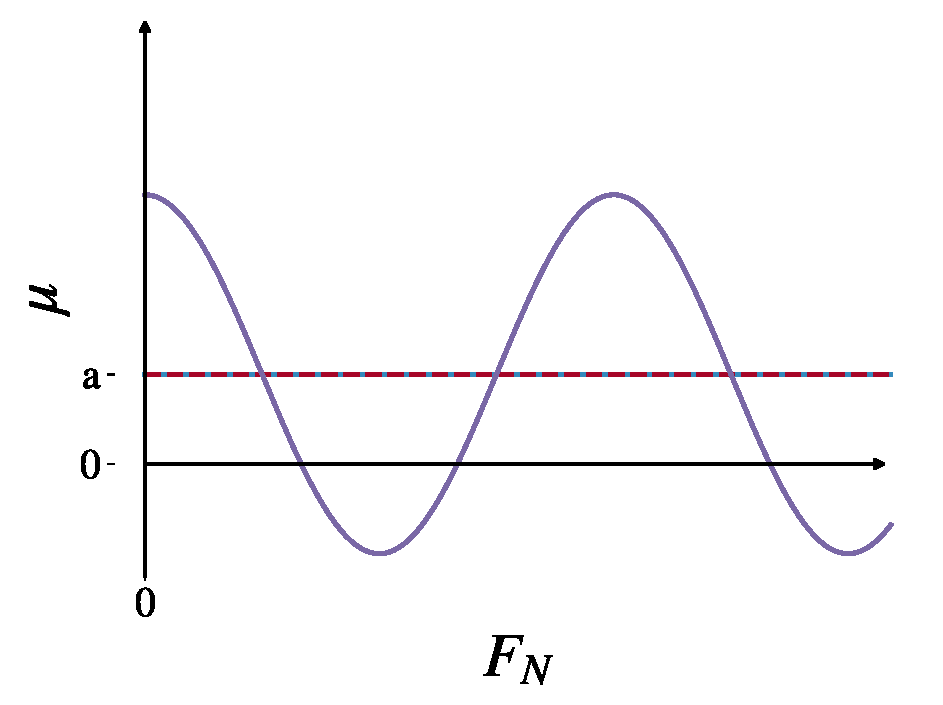
\includegraphics[width=\textwidth]{figures/theory/fric_coef_example_c.pdf}
      \caption{}
      % \label{fig:}
  \end{subfigure}
  \hfill
  \caption{\hl{CAPTION}}
  \label{fig:fric_coef_example}
\end{figure}


Although Amontons' law has been successful in is description of the majority of
rubbing surfaces, involving both dry and lubricated, ductile and brittle and
rough and smooth (as long as they are not adhesive) surfaces \cite{gao_frictional_2004},
it has its limitations. It is now known that \cref{eq:amonton} is not valid
over a large range of loads and sliding velocities and that it completely breaks
down for atomically smooth surfaces in strongly adhesive contact
\cite{gao_frictional_2004}. The independency of sliding velocity dissapears at
low velocities as thermal effects becomes important and for high velocities due
to intertial effetcs \cite[pp. 5-6]{gnecco_meyer_2015}. For the case of static
friction, it was discovered to be dependent on the so-called contact
history with increasing friction as the logarithm of time of stationary contact.

In cases where amontons' law breaks down we might still use the conceptual
definition of the friction coefficient as defined by (\cref{eq:mu_def2}).
Especially, in the context of achieving negative friction coefficients (in certain load ranges) we would refer to this definition, since (\cref{eq:mu_def1}) would imply a truly unphysical situation of the frictional force acting in the same direction as the sliding motion. This would accelerate the object indefinitelly\footnote{You would most likely have a good shot at the Nobel Prize with that paper.}.

Due to the emperical foundation of Amontons’ law it does not provide
any physical insight into the underlying mechanisms of friction. However, as we
will later discuss in more detail, we can understand the overall phenomena of
friction through statistical mechanics by the concept of \textit{equipartition
of energy} \cite{Manini_2016}. A system in equilibrium has its kinetic energy
uniformly distributed among all its degrees of freedom. When a macroscale object
is sliding in a given direction it is clearly not in equilibrium since one of
its degrees of freedom carriers considerable more kinetic energy. Thus, the
system will have a tendency to transfer that kinetic energy to the remaining
degrees of freedom as heat. This heat will dissipate to the sourroundings and
the object will slow down as a result. Hence, we can understand friction simply as the tendency of going toward equilibrium energy equipartitioning among many
interacting degrees of freedom \cite{Manini_2016}. From this point of view it is
clear that friction is an inevitable part of contact physics, but even though
friction cannot be removed altogether, we are still capable of manipulating it in
usefull ways. \\
\\
The attentive reader might point out that we have already moved the discussion
partly into the microscopic regime as \textit{statistical mechanics} generally
aim to explain macroscale behaviour by microscopic interactions. In fact, this 
highlight the nessecity to consider smaller scales in order to achieve a more fundamental understadning of friction.


% All the terms in Amontons’ law refer to macroscopic, i.e., space- and time-averaged or “mean-field”, values. Thus, the contact area is the “apparent” or projected geometric area rather than the “real” contact area at the molecular level. And V is the mean relative velocity of the sliding bodies even though the shearing microjunctions may be moving with large fluctuations or in a stick-slip fashion.10 \cite{gao_frictional_2004}




% This includes taking the microsopic roughness
% into account together with surface chemistry. This more complex perspective
% introduces new (...() as real contact area, contact stresses, surface adhesion
% which makes frictional properties dependent on sliding speed, temperature and
% environment in general \cite{kim_nano-scale_2009}. 


% The conclusion is that the friction coefficient is not an intrinsic physical
% property \cite{Szlufarska_2008}.

% The basic difficulty of friction is intrinsic, involving the dissipative
% dynamics of large systems, often across ill-characterized interfaces, and
% generally violent and nonlinear \cite{Manini_2016}


% The severity of the task is also related to the experimental difficulty to
% probe systems with many degrees of freedom under a forced spatial confinement,
% that leaves very limited access to probing the buried sliding interface.
% Thanks to remarkable developments in nanotechnology, new inroads are being
% pursued and new discoveries are being made. \cite{Manini_2016}


\section{Microscopic scale}
Going from a macro- to microscale perspective, to a length scale of order
\SI{e-6}{m}, it was realized that most surfaces is in fact rough
\cite{mo_friction_2009}. The contact between two surfaces consist of numerous
smaller contact point, so-called asperities, for which the friction between two
opposing surfaces involves interlocking of those asperities as visualized in
\cref{fig:asperity_contact}. Small junctions of asperities are formed due
to contact pressure and adhesion \cite{kim_nano-scale_2009}.

In the macroscale perspective of Amonton's law we refer to time- and
space-averaged values, i.e.\ the ``apparent'' contact area and the average
sliding speed \cite{gao_frictional_2004}. However, microspocially we find the
real contact area to be smaller than the macroscale apparent area and the
shearing of local microjunctions can happen at large fluctuations or in a
stick-slip fashion. 

It is generally accepted that friction is caused by two mechanism: mechanical
friction and chemical friction \cite{kim_nano-scale_2009}. The mechanical
friction is the ``plowing'' of the surface by hard particles or said asperities
with an energy loss attributed to deformations of the asperity. While plastic
deformations, corresponding to wear, gives rise to an obvious attribution for
the energy loss, elastic deformations is also sufficient in explaining energy
loss due to phonon excitations. In fact the assumption of plastic deformations
has been critizised as this is theorized only to be present in the beginning of a
surface contact while it is neglible for prolonged or repeated contact of the same surfaces \cite{CARBONE20082555}. That is, when machine parts slide against each
other for millions of cycle the plastic deformation would only take place in the
beginning for which the system then reaches a steady state with only elastic deformations. The chemical friction arrises from adhesion between microscopic
contacting surfaces, with an energy loss attributed to breaking and forming of
bonds. 



\subsection{Surface roughness --- Asperity theories}
% Sources in general: \cite{mo_friction_2009}, \cite{kim_nano-scale_2009} \\

Asperity theories are based on the observation that microscopic rough surfaces,
with contacting asperities each with a contact area of $A_{\text{asp}}$, will
have a true contact area $\sum A_{\text{asp}}$ much smaller than the apperent
macroscopic area \cite{kim_nano-scale_2009}. The friction
force has been shown to be proportional to the true contact area as 
\begin{align*}
  F_\text{fric} = \vec{\tau} \sum A_{\text{asp}},
\end{align*}

% Adhesion model by Bowden and Tabor. Adhesion is propoertional to asperity contact area giving rise to a proportionality between aperity contact area and interfacial shear strength. \cite{C2NR30691C}
where $\vec{\tau}$ is an effective shear strength of the contacting bodies. Note
that this is still compatible with Amontons’ law in \cref{eq:amonton} by having a linear relatioship between the real contact area and the
applied load. In \cref{fig:asperity_contact} we see a
visualization on how the contact area might intuitively increase with load as the asperity tips is deformed (plastically or elastically) into broader contact points.
\begin{figure}[H]
  \centering
  \begin{subfigure}[b]{0.49\textwidth}
      \centering
      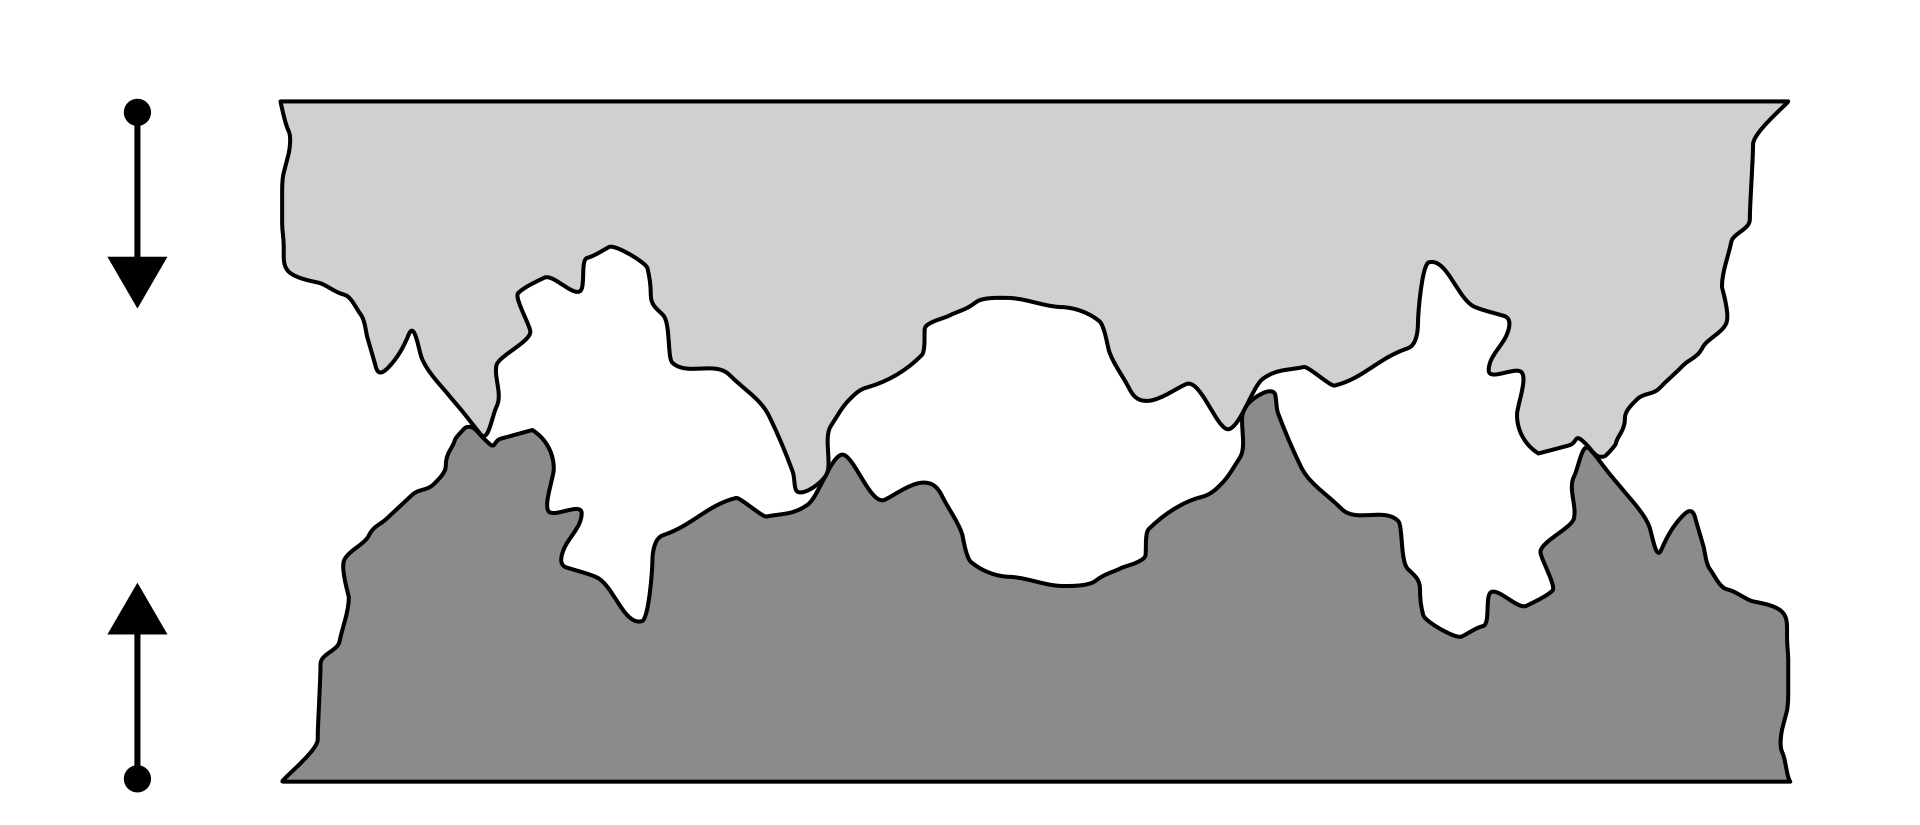
\includegraphics[width=\textwidth]{figures/theory/asperities_top.png}
      \caption{Low load.}
      \label{fig:asp_left}
  \end{subfigure}
  \hfill
  \begin{subfigure}[b]{0.49\textwidth}
      \centering
      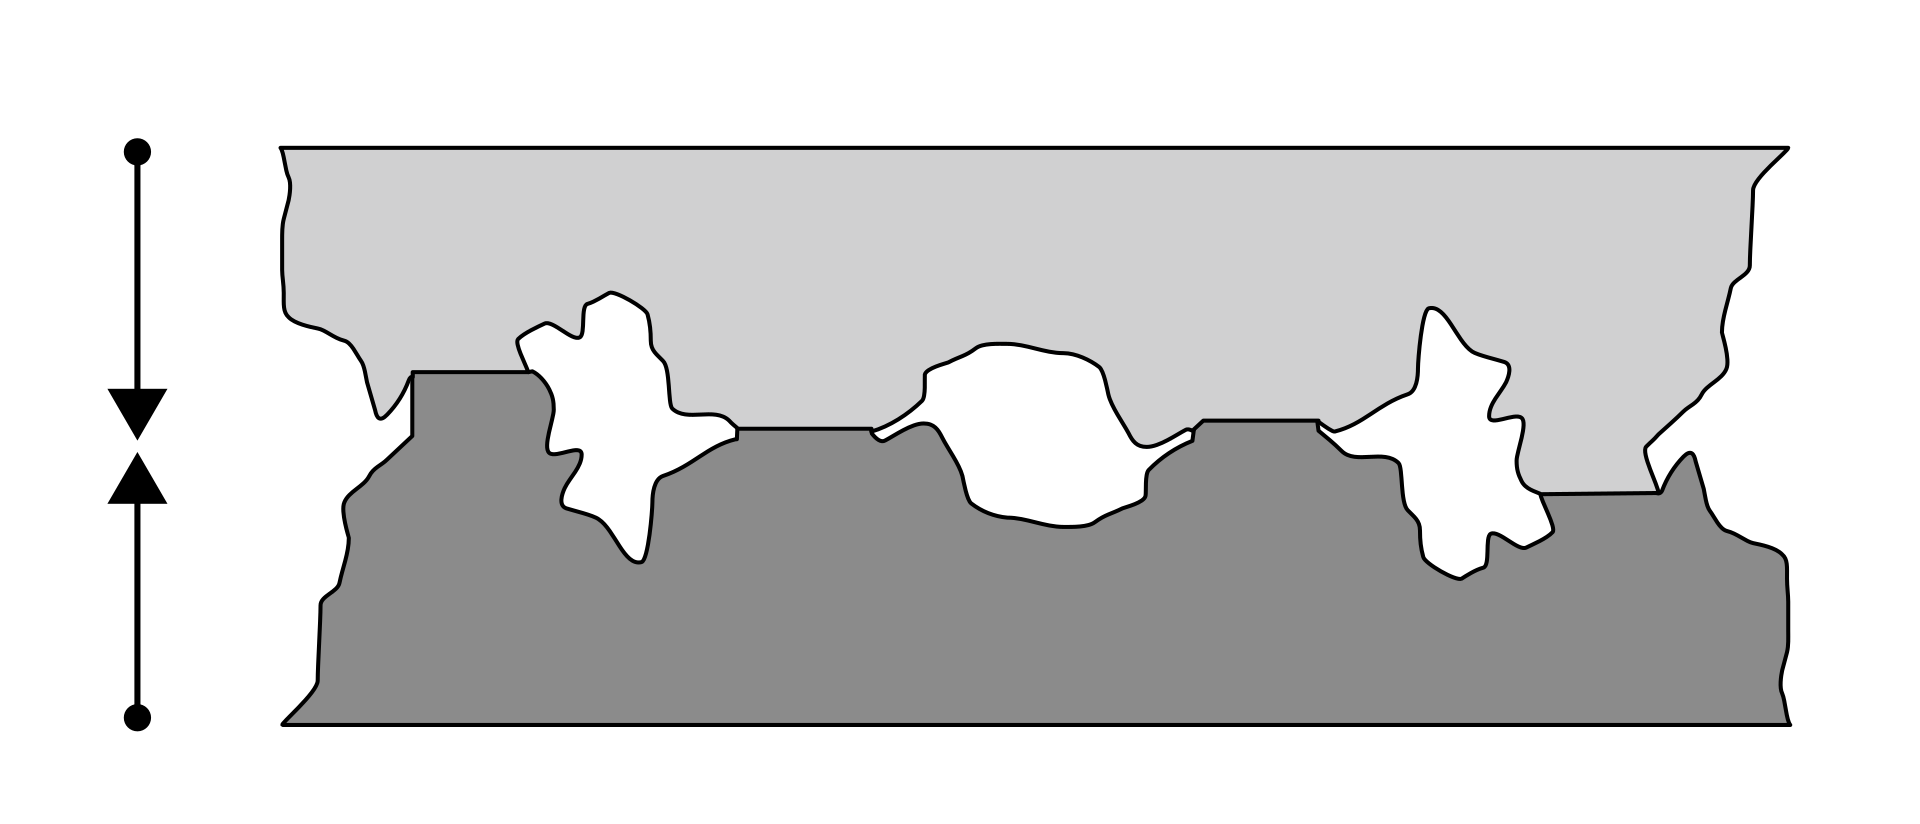
\includegraphics[width=\textwidth]{figures/theory/asperities_bottom.png}
      \caption{High load.}
      \label{fig:asp_right}
  \end{subfigure}
  \hfill
     \caption{Qualitatively illustration of the microscopic asperity deformation
     under increasing load from frame (a) to (b) \cite{wiki:asperities}. While this figure seemingly portrays plastic deformation the concept of increased contact area under increased load applies for elastic deformation as well.}
     \label{fig:asperity_contact}
\end{figure}

Many studies have focused on single asperity contacts to reveal the relationship
between the contact area and load
\cite{Szlufarska_2008}\cite{PhysRevLett.56.930}\cite{perry_scanning_2004}. By
assuming perfectly smooth asperities, with radii of curvature from micrometers
all the way down to nanometers, continuum mechanics can be used to predict the
deformation of asperities as load is applied. A model for non-adhesive contact
between homogenous, isotropic, linear elastic spheres was first developed by
Hertz \cite{HertzOnTC}, which predicted $A_{\text{asp}} \propto F_N^{2/3}$.
Later adhesion effects were included in a number of subsequent models, including
Maugis-Dugdale theory \cite{MAUGIS1992243}, which also predicts a sublinear
relatinship between $A_{\text{asp}}$ and $F_N$. Thus, the common feature of all
single-asperity theories is that $A_{\text{asp}}$ is a sublinear function of
$F_N$, leading to a similar sublinear relationship for $F_\text{fric}(F_N)$,
which fails to align with the macroscale observations modelled by Amontons’ law
(eq. \eqref{eq:amonton}).

% Concurrently with single-asperity studies, roughness contact theories are being developed8–10,16 to bridge the gap between the mechanics of single asperities and that of macroscopic contacts.\cite{mo_friction_2009}

Concurrently with single-asperity studies, roughness contact theories are being developed \cite{PhysRevLett.100.055504}\cite{Persson}\cite{GW}\cite{BUSH197587} to bridge the gap between single asperities and macroscopic contacts \cite{mo_friction_2009}. A variety of multi-asperity theories has attempted to combine single asperity
mechanics by statistical modelling of the asperity height and spatial
distributions \cite{CARBONE20082555}. This has led to a partially success in the establishment of a linear relationship between $A_{\text{asp}}$ and $F_N$. Unfortunately, these results are restricted
in terms of the magnitude of the load and contact area, where multi-asperity
contact models based on the original ideas of Greenwood and Williamson \cite{GW}
only predicts linearity at vanhising low loads, or Persson \cite{Persson} which
works for more reasonable loads but only up to 10-15 \% of the macroscale
contact area. However, as the load is furhter increased all multi-asperity models
predict the contact area to fall into the sublinear dependency of normal force
as seen for single aperity theories as well \cite{CARBONE20082555}.


% Da Vinci-Amontons law – friction independent of area – is not confirmed at the
% microscopic scale. In most nanoscale investigations the friction of a single
% con- tact is found to increase linearly with the contact area [27–29]. In
% contrast, structurally mismatched atomically flat and hard crystalline or
% amorphous surfaces are expected to produce a sublinear increase of friction
% with contact area. The frequent finding of friction proportional to area even
% in some of these cases can be understood as a consequence of softness, either
% if the interface, or of surface contaminants leading to effectively pseudo-
% commensurate interfaces [30, 31] (Current trends in the physics of nanoscale
% friction)


% Other authors proposed an empirical model in which mechanics of a nanoscale non-adhesive contact is controlled by load, that is, $F_f = \mu L$ and the contact area is undefined and unnecessary5,29 \cite{mo_friction_2009}

% \cite{mo_friction_2009} agues that the break-down of single-asperity theories of friction is due to the asperity (circumfereance defined) area is not proportional to the real one. By obtaining the real area (contacting bond) he arrives at the macroscale relationship... Quote: As shown in Table 1, friction force is now proportional to contact area at all length scales as long as the contact area is correctly defined at each length scale. When adhesion is added they arrive at the sublinear trend again. 


% \hl{What about multi asperity theory?}

% Our model predicts that as the adhesion between the contacting surfaces is reduced, a transition takes place from nonlinear to linear dependence of friction force on load. \cite{mo_friction_2009}




% This approach enables the bottom-up derivation of the linear scaling laws of macroscopic friction with size, and their transition to the sublinear ones for incommensurate nanosized contacts. We can now understand that such transition takes place when the contact roughness becomes large compared to the range of interfacial interactions [162] \cite{Manini_2016}.


% However, practical single- and multiplecontact conditions are characterized by
% complex interaction profiles plus nontrivial internal dynamics. As a result,
% the interplay of thermal drifts, contact ageing, contact-contact interactions,
% and macroscopic elastic deformations introduce significant complications, and
% make the depinning transition from static to kinetic friction an active field
% of research. \cite{Manini_2017}[p. 2]. 



% However, even though the successes of continuum mechanics there is no reasion to
% believe that it will be capable of reproducing tribological behaviour at the
% nanometre length scale where the discreteness of atoms often has a direct effect
% on physical properties \cite{Szlufarska_2008}.


\section{Nanoscale - Atomic scale}
Going from a micro- to a nanoscale, on the order of \SI{e-9}{m}, it has been
predicted that continnum mechanics will break down \cite{luan_breakdown_2005}
due to the discreteness of individual atoms. Note that atom spacing lies in the
domain of a few ångströms Å (\SI{e-10}{m}) and thus we take the so-called atomic-scale to be a part of the nanoscale regime. In a numerical
study by Mo et al.\ \cite{mo_friction_2009} (considering asperity radii of 5-30
nm) it has been shown that the asperity area $A_{\text{asp}}$, defined by the
circumfereance of the contact zone, is sublinear with
$F_N$. This is accommodated by the observation that not all atoms within the
circumfereance make chemical contact with the substrate. By
modelling the real contact area $A_{\text{real}} = NA_{\text{atom}}$, where $N$ is the amount of atoms within the range of chemical interaction and
$A_{\text{atom}}$ the associated surface area for an atom, they found a consistent
linear relationship between friction and the real contact area. Without adhesive
forces this lead to a similar linear relationship $F_{\text{fric}} \propto F_N$,
while adding van der Waals adhesion to the simulation gave a sublinear
relatinship, even though the $F_{\text{fric}} \propto A_{\text{real}}$ was
maintained. This result emphasizes that the contact area is still expected to be play an important role at the nanoscale for asperity theory. It is simply the definition of the contact area that undergoes a change when transistioning from micro- to nanoscale. 


% Refer to the system introduced in Introduction

While the study by Mo et al.\ \cite{mo_friction_2009} considers a single
asperity on a nanoscale, we are going to study a nanoscale system with no
initial asperities present. Our system of interest, an initially atomically flat graphene sheet imposed on a flat silicon substrate, make it unfounded to rely on asperity theories. Although both numerical \cite{zhu_study_2018}\cite{ma12091425}\cite{bonelli_atomistic_2009} and experimental \cite[2005]{DIENWIEBEL2005197}\cite{feng_superlubric_2013} studies have been done for so-called nanoflakes
sliding on a substrate, the dependence of friction force on contact area is not investigated.  One reasonable explanation is that the contact area is already at its maximum for atomically smooth contacting surfaces and hence does not play an important role. In a numerical study of atomic-scale frictional behavior of corrugated nano-structured surfaces \cite{C2NR30691C} they reported that the contact area only affected the friction significantly for big corrugations as opposed to small. Since an increasing friction is still reported under increasing load in most nanoflake studies (see
\cref{sec:expected_prop} for a more detailed dicussion), this suggests
that some other mechanisms are governing friction at this level. 

Before diving into alternative theoretical approaches to adress this issue we point out that exactly this transistion, between nanoscale asperities and atomically smooth surfaces, is of outermost importance for the objective of the thesis. By introducing kirigami cuts and stretching the sheet we expect to see an out of plane buckling which induce an ensemble of asperities on the sheet. Hence, we might hypothesize that such a transition will contribute to a significant change in the goverening mechanism of friction bridgering the two domains of nanoscale asperity and smooth surface theory. 
\\
\\
In the lack of noteworthy structural asperities, friction can instead be
modelled as a consequencse of the rough potential of the atomic landscape. A
series of models builds on this idea by considering different ways for the atoms
to interact interatomically, with the moving body, and the substrate. In figure
\cref{fig:PT_FK_FKT} three of the most common 1D models is displayed. The
time-honered Prandtl-Tomlinson (PT) model describes a point-like tip sliding
over a space-periodic fixed crystalline surface with a harmonic coupling to the
moving body. This is analog to that of an experimental cantilever used
for Atomic Force Microscopy (see \cref{sec:SPM}). Further extensions was
added in the Frenkel-Kontorova (FK) model by substituting the tip with a chain
of harmonic coupled atoms dragged from the end (\hl{I am not sure that the figure is 100\% correct by drawing a spring like that}), and finally combinned
in the Frenkel-Kontorova-Tomlinson (FKT) with the addition of a harmonic
coupling between the chain and the moving body. In the following we will disucss the FK model as the underlying basis for the understanding of smooth nanoscale friction.

\begin{figure}[H]
  \centering
  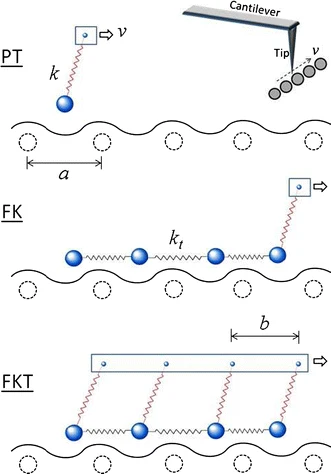
\includegraphics[width=0.4\linewidth]{figures/theory/PT_FK_FKT.png}
  \caption{\hl{Temporary} figure from \url{https://www.researchgate.net/figure/llustrations-of-the-1D-PT-FK-and-FKT-models-Large-solid-spheres-represent-tip-atoms_fig1_257670317}}
  \label{fig:PT_FK_FKT}
\end{figure}




% Our results confirm the conclusions of other authors that single-asperity theories break down at the nanoscale1,5. \cite{mo_friction_2009}


% Experimental research to examine the frictional characteristics at the
% atomic-scale has been conducted for the past two decades. It is well known
% that frictional behavior cannot be generalized by a few factors such as normal
% load, surface roughness, speed, and material type of the tribological system.
% Other conditions such as temperature, humidity, and even sliding history can
% affect the tribological phenomena significantly. Particularly at nano-scale,
% the tribological behavior tends to be more sensitive to the state of outermost
% layer of the surface region. Thus, contamination layer, adsorbed gas,
% capillary junctions, and oxide layer become more important at small scales.
% This is because at nano-scale the contact forces are often too low for the
% asperities to penetrate the surface layers and the magnitude of the surface
% force may be comparable to the frictional force. {kim_nano-scale_2009}.


% Together with the current experimental possibility to perform well-defined
% measurements on well-characterized materials at the fundamental microscopic
% level of investigation of the sliding contacts, advances in the computer
% modeling of interatomic interactions in materials science and complex systems
% encompass molecular-dynamics (MD) simulations of medium to large scale for the
% exploration of the tribo-dynamics with atomic resolution [4, 5].




% \subsection{Tomlinson model}
% % \cite{kim_nano-scale_2009}

% One of the first atomic scale models. Here we have no asperities but it is based on the assumptions that the atomic surface is not completely smooth. Since atoms was modelled as spheres the surface topography would not be completely flat. The idea is shown in \cref{fig:tomlinson_model} where the moving body is connected the atom with springs.
% \begin{figure}[H]
%   \centering
%   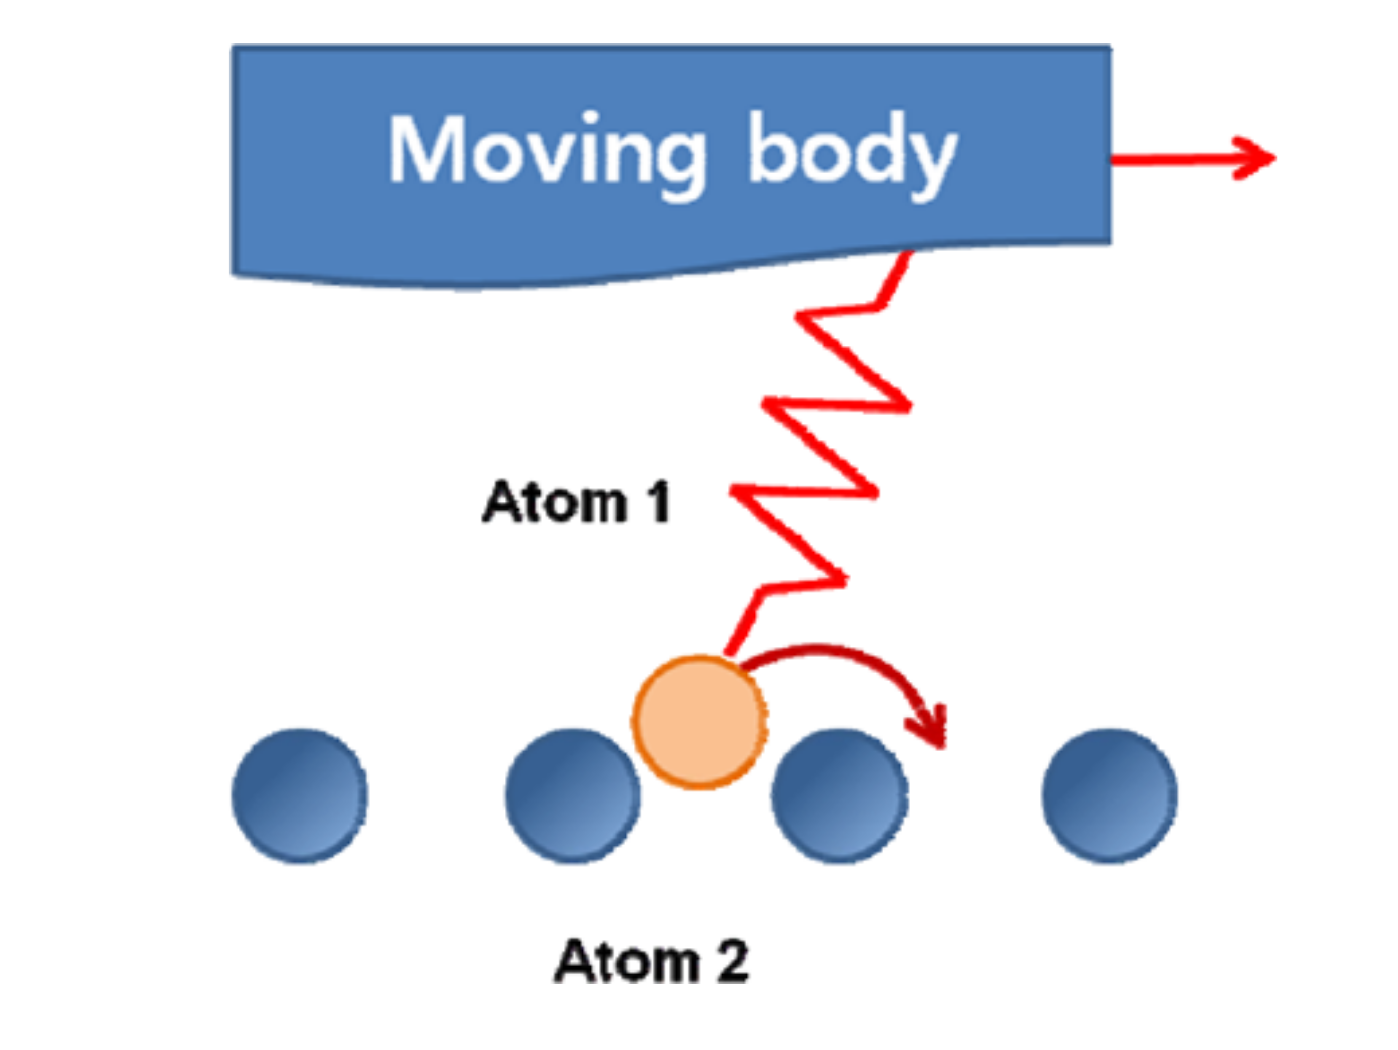
\includegraphics[width=0.5\linewidth]{figures/theory/tomlinson_model.png}
%   \caption{\hl{Temporary} figure from \cite{kim_nano-scale_2009}}
%   \label{fig:tomlinson_model}
% \end{figure}


% This model gives an explanation to the stick-slip behaviour. This layed the foundation for the Frenkel-Kontorova model so maybe go straight to that?

\subsection{Frenkel-Kontorova}
% Based on \cite{Manini_2016} and \cite{FK2D}.

The standard Frenkel-Kontorova (\acrshort{FK}) model consists of a 1D chain of $N$ classical
particles of equal mass, representing atoms, interacting via hamornic forces and moving in a sinusoidal potential as sketched in \cref{fig:FK_model} \cite{Manini_2016}. The hamiltonian is 
\begin{align}
  H = \sum_{i=1}^N \left[\frac{p_i^2}{2m} + \frac{1}{2}K(x_{i+1} - x_i - a_c)^2 + \frac{1}{2}U_0 \cos{\left(\frac{2\pi x_i}{a_b}\right)}\right],
  \label{eq:H_FK}
\end{align}
where the atoms are labelled sequently $i = 1, \hdots, N$. The first term $p_i^2/2m$ represents the kinetic energy with momentum $p_i$
and mass $m$. Often the effetcs of inertia are neglected, reffered to as the static \acrshort{FK} model, while the inclusion in \cref{eq:H_FK} is known as the dynamic \acrshort{FK} model \cite{FK2D}. The next term describes the harmonic interaction with elastic
constant $K$, nearest neighbour distance $\Delta x = x_{i+1} - x_i$ and 
corresponding nearest neighbour equilibrium distance $a_c$. The final term represents the periodic substrate potential, serving as the external potential on site, with amplitude $U_0$ and period $a_b$. Different boundary choices can be made where both free ends and periodic conditions gives similar results. The choice of fixed ends however makes the chain incapable of sliding.

\begin{figure}[H]
  \centering
  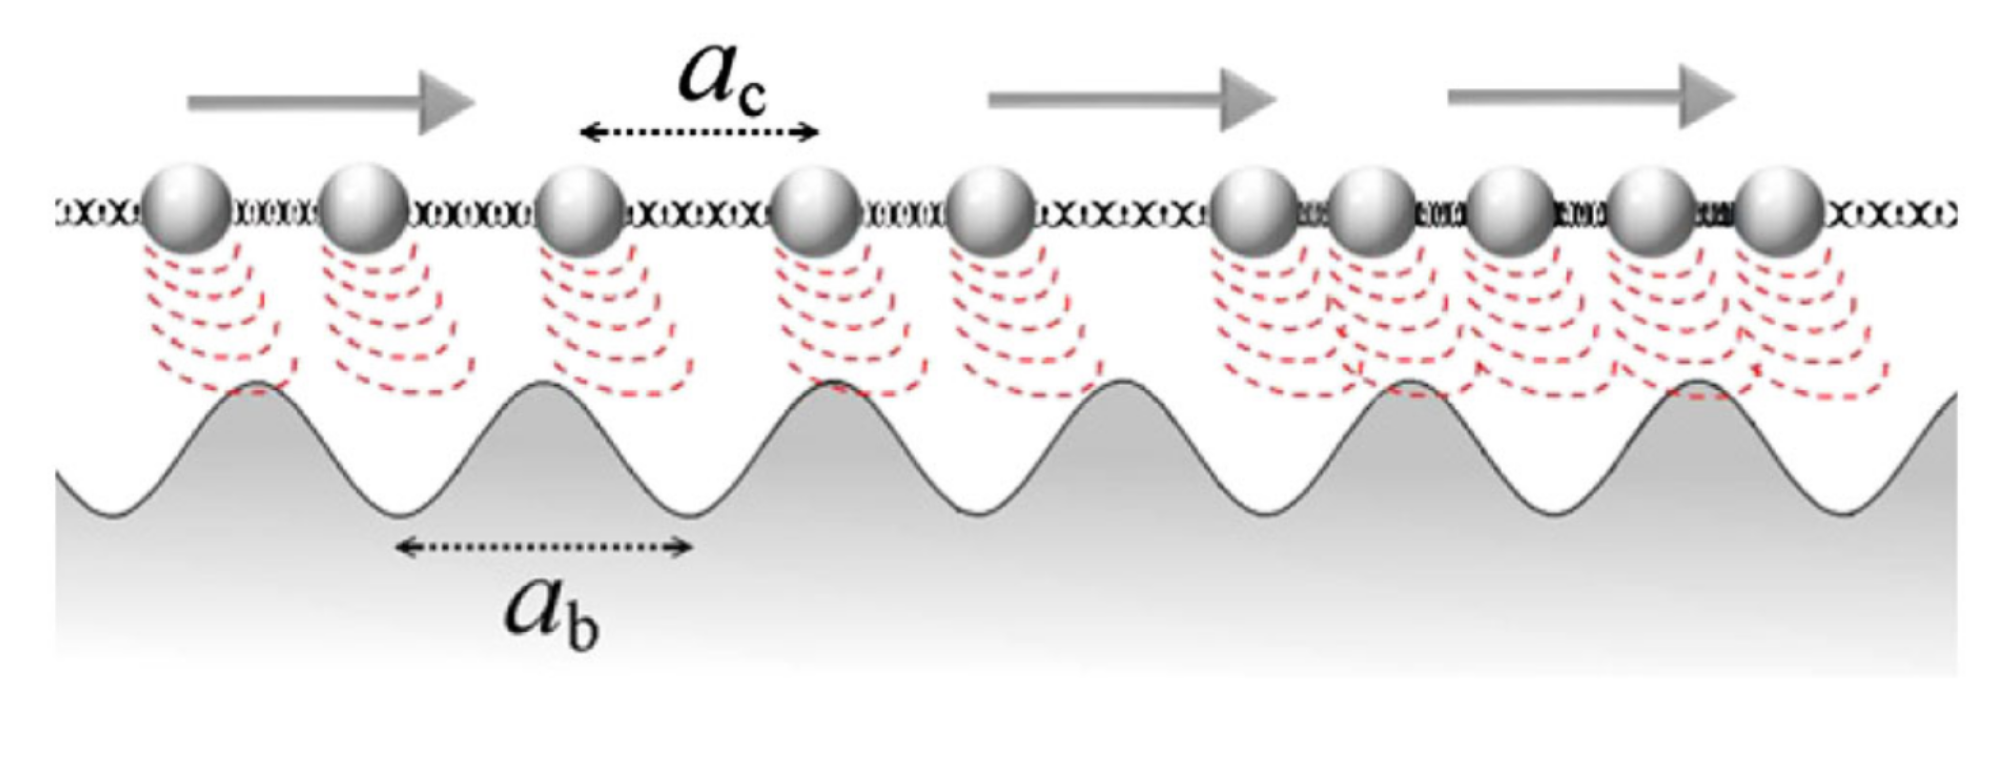
\includegraphics[width=0.8\linewidth]{figures/theory/FK_model.png}
  \caption{\hl{Temporary} figure from \cite{Manini_2016}}
  \label{fig:FK_model}
\end{figure}

To probe static friction one can apply an external adiabatically increasing force until sliding accours. This corresponds to the static \acrshort{FK} model, and it turns out that the sliding properties are entirely governed by its topological excitations referred to as so-called \textit{kinks} and \textit{antikinks}

\subsubsection{Commensurability} We can subdivide the frictional behaviour in terms of commensurability, that is, how well the spacing of the atoms match the periodic substrate potential. We describe this by the length ratio $\theta = a_b / a_c = N / M$ where $M$ denotes the number of minemas in the potential (within the length of the chain). A rational number for $\theta$ means that we can achieve a perfect alignment between the atoms in the chain and the potential minemas, without stretching the chain, corresponding to a \textit{commensurate} case. If $\theta$ is irrational the chain and substrate cannot fully align without some stretching of the chain, and we denote this as being \textit{incommensurate}.

We begin with the simplest commensurate case of $\theta = 1$ where the spacing
of the atoms matches perfectly with the substrate potential periodicity, i.e.\
$a_c = a_b$, $N = M$. The ground state (\acrshort{GS}) is the configuration where each atom
is aligned with one of the substrate minema. By adding an extra atom to the chain we would effectively shift some of the atoms out of this ideal state, giving rise to a kink excitation. This leads to the case where two atoms will have to ``share'' the same potential corrugation as sketched in \cref{fig:incommensurable_example}.  On the
other hand, removing an atom from the chain results in an antikink excitation
where one potential corrugation will be left ``atomless''. In order to reach a
local minimum the kink (antikink) will expand in space over a finite length such
that the chain undertakes a local compression (expansion). When applying a
tangential force to the chain it is much easier for an excitation to move along
the chain than it is for the non-exicted atoms since the activation energy
$\epsilon_{PN}$ for a kink/antikink displacement is systematically smaller
(often much smaller) than the potential barrier $U_0$. Thus, the motion of kinks
(antikinks), i.e.\ the displacement of extra atoms (atom vacancies), is
represententing the fundamental mechanism for mass transport. These
displacements are responsible for the mobility, diffusivity and conductivity
within this model. 

In the zero temperature commensurable case with an adiabatical increase in force, all atoms would be put into an accelerating motion as soon as the potential barrier energy is present. However, in reality any thermal excitation would excite the system before this point is reached resulting in kink-antikink pairs traveling down the chain. For a chain of finite length these often accour at the end of the chain running in opposite direction. As a kink travels down the chain the atoms are advanced by one lattice spacing $a_b$ along the substrate potential. This cascade of kink-antikink exications is shown in \cref{fig:kink_antikink}

\begin{figure}[H]
  \centering
  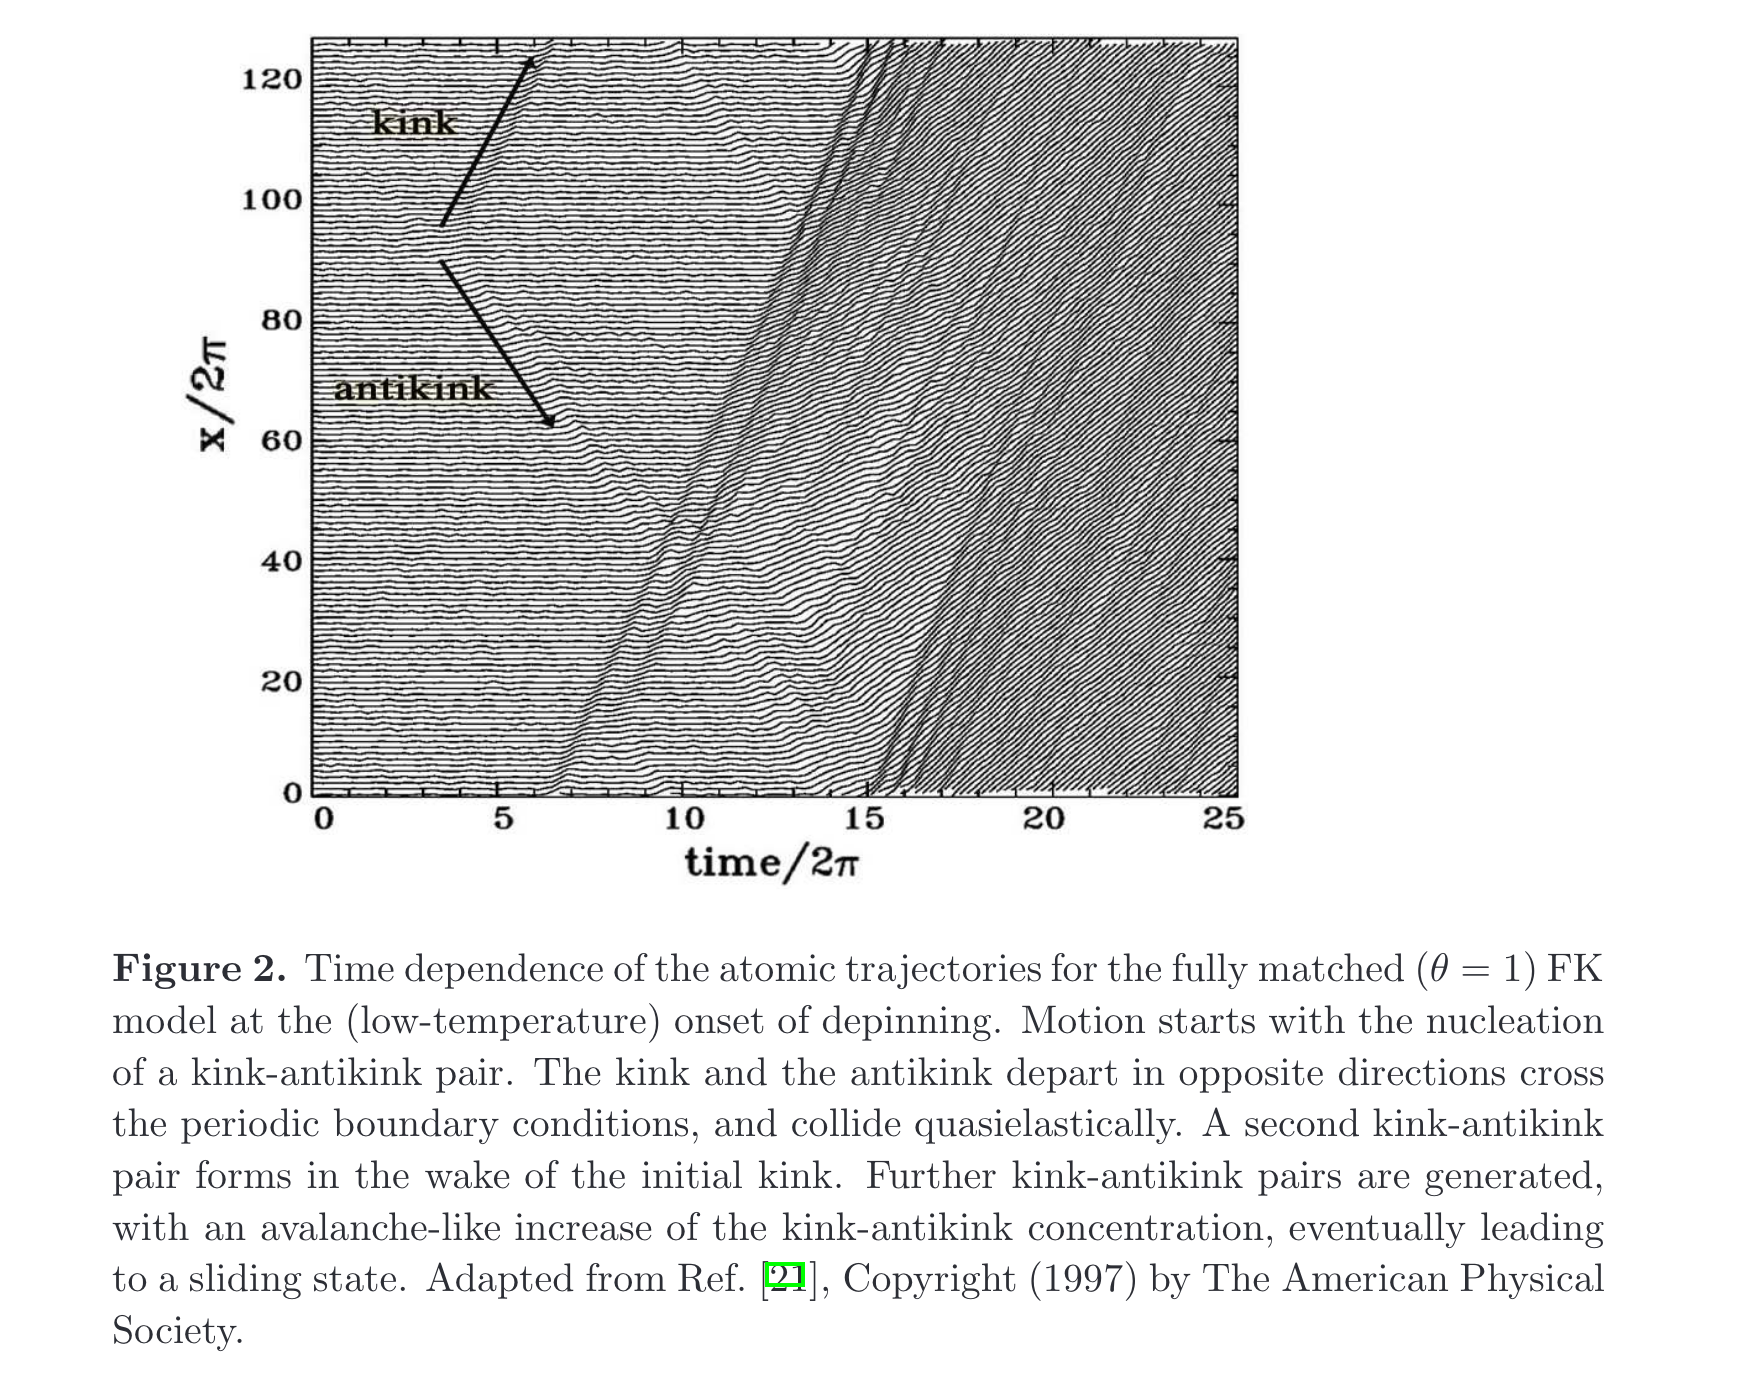
\includegraphics[width=0.8\linewidth]{figures/theory/kink_antikink.png}
  \caption{\hl{Temporary} figure from \cite{Manini_2016}}
  \label{fig:kink_antikink}
\end{figure}

For the 2D case where an island (or flake) is deposited on a surface, in our case the graphene sheet on the Si substrate, we generally also expect the sliding to be initated by kink-antikink pairs at the boundary. 

For the case of incommensurability, i.e.\ $\theta = a_b/a_c$ is irrational, the
\acrshort{GS} is characterized by a sort of ´´staircase'' deformation. That is, the chain will exhibit regular periods of regions where the chain is slightly compressed
(expanded) to match the substrate potential, seperated by kinks (antikinks),
where the increased stress is eventually released 
% through a localized expansion (compression) 
as illustrated in \cref{fig:incommensurable_example} 
% \hl{Go through this last part  again. Even though this is what the source says I'm not quite sure I understand why it is not opposite ``...released through a localized compression (expansion)''?}.

\begin{figure}[H]
  \centering
  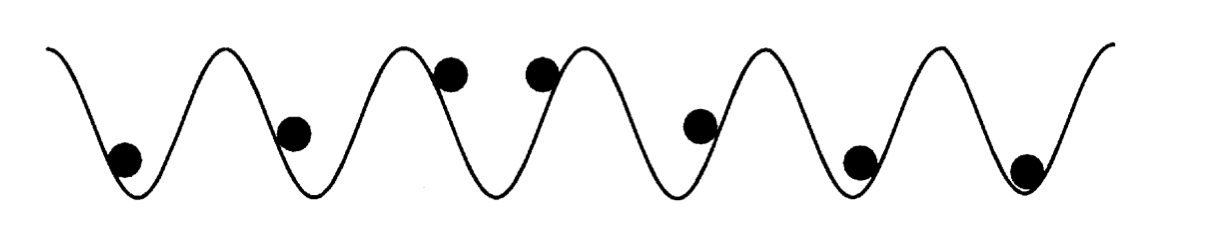
\includegraphics[width=0.5\linewidth]{figures/theory/incommensurable_example.png}
  \caption{\hl{Temporary} figure from
  url{http://www.iop.kiev.ua/~obraun/myreprints/surveyfk.pdf} p. 14.
  Incommensurable case ($\theta = ?$) where atoms sits slightly closer than
  otherwise dictated by the substrate potential for which this regularly result
  in a kink here seen as the presence of two atoms closely together in on of the
  potential corrugations.}
  \label{fig:incommensurable_example}
\end{figure}

% Maybe use the strength $\lambda = U_0 / (K a_b^2)$ with critical strength $\lambda_c$ instead of critical $K$?

The incommensurable \acrshort{FK} model contains a critical elastic constant $K_c$, such
that for $K > K_c$ the static friction $F_s$ drops to zero, making the chain able to initiate a slide at no energy cost, while the low-velocity kinetic friction is dramatically reduced. This can be explained by the
fact that the displacement accouring in the incommensurable case will yield just
as many atoms climbing up a corrugation as there are atoms climbing down. For a big (infinite) chain this will exactly balance the forces making it
non-resistant to sliding. Generally, incommensurability guarantees that the
total energy (at $T=0$) is independent of the relative position to the
potential. However, when sliding freely a single atom will eventually occupy a
maximum of the potential. When increasing the potential magnitude $U_0$ or
softning the chain stiffness, lowering $K$, the possibility to occupy such a
maximum dissapears. This marks the so-called \text{Aubry transition}
at the critical elastic constant $K = K_c(U_0, \theta)$ where the chain goes
from a free sliding to a \textit{pinned state} with a nonzero static friction.
$K_c$ is a discontinuous function of the ratio $\theta$, due to the reliance on
irrational numbers for incommensurability. The minimal
value $K_c \simeq 1.0291926 $ in units $[2 U_0 (\pi / a_b)^2]$ is achieved for
the golden-mean ratio $\theta = (1+\sqrt{5}/2)$. Notice that the pinning is
provided despite translational invariance due to the inaccessibility to move
past the energy barrier which act as a dynamical constraint. The Aubry transistion
can be invistigated as a first-order phase transistion for which power laws can be
defined for the order parameter, but this is beyond the scope of this thesis.
%  This is beyond the scope of this thesis as we
% merely are going to point to the \acrshort{FK} model for the understanding of stick-slip behvaiour and the concept of commensurability.

The phenonema of non-pinned configurations is named \textit{superlubricity} in
tribological context. Despite the misleadning name this referes to the case
where the static friction is zero while the kinetic friction is nonzero but
reduced. For the case of a 2D sheet it is possible to alter the commensurability, not only by changing the lattice spacing through material choice, but also
by changing the orientation of the sheet relative to the substrate. Dienwiebel et al.\ \cite{DIENWIEBEL2005197} have shown that the kinetic friction, for a graphene flake sliding over a graphite surface (multiple layers of graphene), exhibits extremely low friction at certain orientations as shown in \cref{fig:graphene_rot}. We clearly see that friction changes as a function of orientation angles with only two spikes of considerable friction force.

\begin{figure}[H]
  \centering
  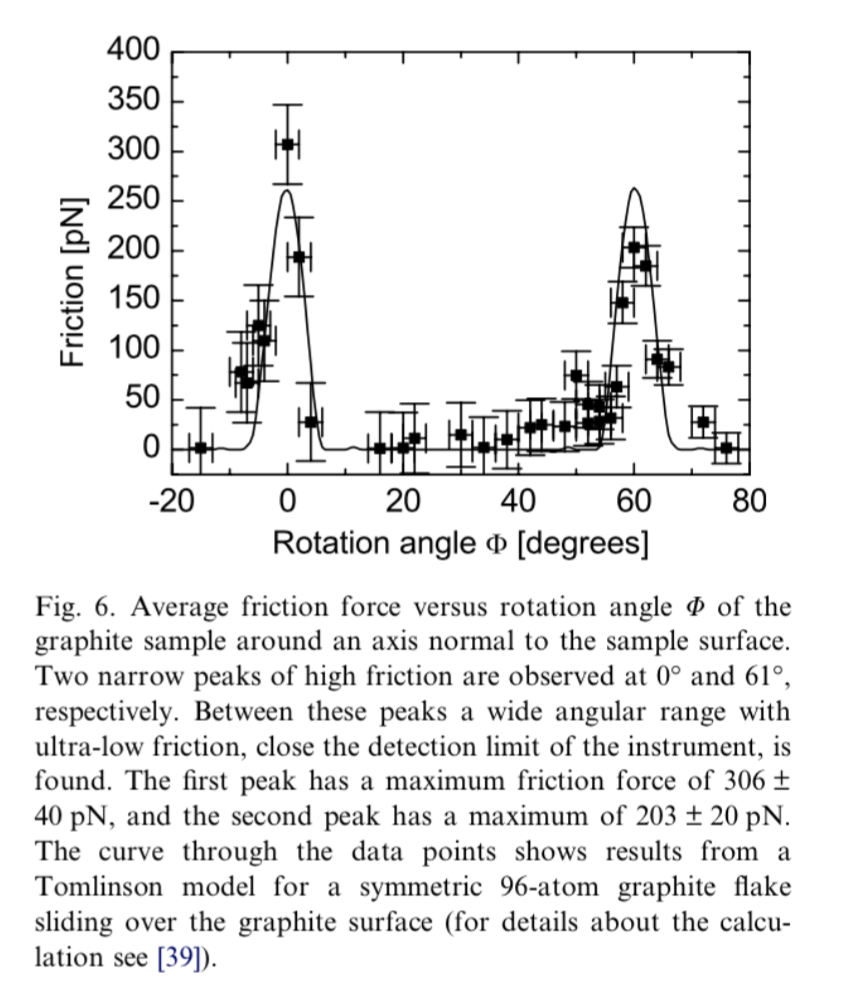
\includegraphics[width=0.5\linewidth]{figures/theory/graphene_rot.png}
  \caption{\hl{Temporary} figure from \cite{DIENWIEBEL2005197} showing superlubricity for incommensurable orientations between graphene and graphite. \hl{temporary}}
  \label{fig:graphene_rot}
\end{figure}





\subsubsection{Kinetic friction}
% Maybe check out for more info on the 1D model: Y. S. Kivshar O. M. Braun. The Frenkel-Kontorova Model. Springer, 1st edition, 2004.
% The Frenkel-Kontorova Model.pdf p. 38 3.2 Dynamics of Kinks <---------

%Based on \cite{FK2D}


% The \acrshort{FK} model can also describe phonons and heat in the lattices, which absorb the kinetic energy of the sliding[4]. \cite{FK2D}

% Consequently, the \acrshort{FK} model is the simplest model in which dynamic friction is emergent, while in other models some form of heuristic damping must be included.\cite{FK2D}

In the \acrshort{FK} model the kinetic friction is primarily caused by resonance between
the sliding induced vibrations and phonon modes in the chain \cite{FK2D}. The specific dynamics is found to be highly model and dimension specific, and even for the 1D case this is rather complex. However, we make a simplified analysis of the 1D rigig chain case to showcase the reasoning behind the phenomena.

When all atoms are sliding rigidly with center of mass velocity $v_{{\text{CM}}}$ the atoms will pass the potential maxima with the so-called \textit{washboard frequency} $\Omega = 2\pi v_{{\text{CM}}} / a_b$. For a weak coupling between the chain and the potential we can use the zero potential case as an approximation for which the known dispersion relation for the 1D harmonic chain is given \cite[p. 92]{Kittel2004}
\begin{align*}
  \omega_k = \sqrt{\frac{4 K}{m}} \left|\sin{\left(\frac{k}{2}\right)}\right|,
\end{align*}
where $\omega_k$ is the phonon frequency and $k = 2\pi i / N$ the wavenumber with $i\in [N/2, N/2)$. Resonance will accour when the washboard frequency $\Omega$ is close to the frequency of the phonon modes $\omega_q$ in the chain with wavenumber $q = 2\pi a_c / a_b = 2\pi \theta^{-1}$ or its harmonics $nq$ for $n = 1, 2, 3, \hdots$ \cite{van_den_Ende_2012}. Thus, we can approximate the resonance center of mass speed as
\begin{align*}
    n \Omega &\sim \omega_{nq} \\
    n \frac{2\pi v_{\text{CM}}}{a_b} &\sim \sqrt{\frac{4K}{m}} \left| \sin{\left(\frac{2n \pi \theta^{-1}}{2}\right)}\right| \\
    v_{\text{CM}} &\sim \frac{\sin{(n\pi \theta^{-1})}}{n \pi} \sqrt{\frac{Ka_b^2}{m}}.
\end{align*}
When the chain slides with a velocity around resonance speed, the washboard
frequency can excite acoustic phonons which will dissipate to other phonon modes
as well. At zero temperature the energy will transform back and forth between
internal degrees of freedom and center of mass movement of the chain. Hence, at
zero temperature this is in fact theorized to speed up the translational decay \cite{FK2D}.
However, for the more realistic case of a non-zero temperature the substrate
serves as a thermostat, for which energy will dissipate from the chain to the
substrate degrees of freedom, giving rise to kintetic friction. This suggets
that certain sliding speeds will exhibit relatively high kinetic friction while
others will be subject to extremely low kinetic friction. Simulations of
concentric nanotubes in relative motion (telescopic sliding) have revealed the
occurence of certain velocities at which the friction is enhanced, corresponding
to the washboard frequency of the system \cite{Manini_2016}. The friction
response was observed to be highly non-linear as the resonance velocities were
approached. 

% This is strongly connected to the superlubricity term, although the phonon
% dynamics in this analysis is overly simplified, and additionaly we expect more
% complex resonance dynamics for higher dimensions. 

A common way to model the non-zero temperature case is by the use of a Langevin
thermostat, which models the dissipation of heat by adding a viscous damping
force and thermal fluctuations by the addition of Gaussian random forces with
variance proportional to the temperature (see \cref{sec:langevin} for more details). In combination, this gives rise to a kinetic
friction that is both velocity and temperature dependent. By extending the \acrshort{FK} model into 2D \cite{FK2D} it can be shown numerically that
the friction coefficient generally increases with increasing velocity and
temperature resepectively, although the specific of the trend is highly
sensitive to model parameters. 


% Simulations of concentric nanotubes in relative motion (telescopic sliding), have revealed the occurrence of well-defined velocities at which friction is enhanced, corresponding to a washboard frequency resonating with longitudinal [172] or circular [173] phonon modes, leading to enhanced energy dissipation. The frictional response becomes highly non-linear while approaching the critical velocity and, contrary to macroscopic systems, washboard resonances can arise at multiple velocities, especially for incommensurate interfaces where more than one length scale may be in common to the contacting surfaces [172] \cite{Manini_2016}.




% As the system is Hamiltonian (no heuristic damping) the total energy is conserved. Nevertheless, energy can be transferred from the centre of mass to the internal degrees of freedom, leading to the arrest of the chain in time. This effect can be interpreted as an effective friction. \cite{van_den_Ende_2012}


% The majority [6–12] examines the steady state of the dynamical \acrshort{FK} model in the presence of dissipation, rep- resenting the coupling of phonons to other, undescribed degrees of freedom. \cite{PhysRevLett.85.302}


% Static friciton behvaiour is robust and remains similar in 2D but dynamical friction is strongly influenced. 




% When considering the nonzero temperature thermal fluctuations can then overcome pinning effects even in fully commensurate cases.



% By applying a finite driving force it is known that a pinned configuration will go through several first-order dynamical pahse transistions as the system transfers from a pinned to a sliding state. 



% At face value, the transition from a static strained configuration to full
% sliding is conceptually as simple as overcoming an energy barrier. However,
% practical single- and multiple- contact conditions are characterized by
% complex interaction profiles plus nontrivial internal dynamics. As a result,
% the interplay of thermal drifts, contact ageing, contact-contact in-
% teractions, and macroscopic elastic deformations introduce significant
% complications, and make the depinning transition from static to kinetic
% friction an active field of research. The depinning dynamics affects in
% particular the transition between stick-slip and smooth slid- ing for sliding
% friction. (Current trends in the physics of nanoscale friction)


% In Atomic Force Microscopy (AFM) experiments, when the tip scans over the
% monolayers at low speeds, friction force is reported to increase with the
% logarithm of the velocity, similar to that observed when the tip scans across
% crystalline surfaces. This velocity dependence is interpreted in terms of
% thermally activated depinning of interlocking barriers involving interfacial
% atoms. (Current trends in the physics of nanoscale friction)




% \begin{enumerate}
%   \item Properties depending on $\Theta = N/M = a_b/a_c$
%   \item Elastic constant $K$
%   \item Kinks anti kinks travelling
%   \item Importance of commensurability between lattice and potential 
%   \item Aubry transition
%   \item Pinning and unpinning, stick slip
%   \item superlubricity (no stick slip, but still kinetic friction)
%   \item Adding a Langevin thermostat on top of this introduces temperature. 
%   \item Phase transistion?
% \end{enumerate}







% \subsection{FK extension: Frenkel-Kontorova-Tomlinson (FKT)}

% Further model extensions. Important? 
% Several extensions has been provided for the FK model with modifications of the
% interactions or system dimensionality. Anharmonicity of the chain 


% However, Weiss and Elmer (1995) proposed that the model had a deficiency. They suggested that in the FK model, there was no connection between the atoms and the sliding body. Therefore, Frenkel-Kontorova-Tomlinson (FKT) model that combines the FK model with the Tomlinson model was proposed. \cite{kim_nano-scale_2009}


% The Frenkel-Kontorova-Tomlinson (FKT) model [61, 62] introduces an harmonic
% coupling of the sliding atomic chain to a driving support, thus making it
% possible to investigate stick-slip features in a 1D extended simplified
% contact. The FKT framework provided the ideal platform to investigate the
% tribological consequences of combined interface incommensurability,
% finite-size effects, mechanical stiffness of the contacting materials, and
% normal-load variations \cite{Manini_2016}.


% Important generalizations involving increased dimensionality compared to the
% regular FK model bear significant implications for tribological properties
% such as critical exponents, size-scaling of the friction force, depinning
% mechanisms, and others. \cite{Manini_2016}

% Maybe check this out: An interesting example of such a transient is the
% depinning of an atomic monolayer driven across a 2D periodic substrate profile
% of hexagonal symmetry [83].  \cite{Manini_2016}


% \subsection{Other stuff}


% At nanoscales things get a bit more unclear. SFM (explain) experiments have
% reported (copy sources 5, 6, 21 from \cite{mo_friction_2009}) where $F_f \propto
% F_N$ or even with these quantities being nearly independent of each other.

% \cite{physicsworld_2005}

% Physically relevant quantities, including the average friction force, the slider and the lubricant mean velocities, several correlation functions, and the heat flow can be evaluated numerically by carrying out suitable averages over the model dynamics of a sliding interface, as long as it is followed for a sufficiently long time. The modeling of friction must first of all address correctly ordinary equilibrium and near-equilibrium phenomena, where the fluctuation-dissipation theorem (Sec. 2) governs the smooth conversion of mechanical energy into heat, but most importantly it must also deal with inherently nonlinear dissipative phenomena such as instabilities, stick-slip, and all kinds of hysteretic response to external driving forces, characteristic of non-equilibrium dynamics. 
% \cite{Manini_2016}


% In several works by J. Fineberg’s group [2–4] the transition from sticking to
% sliding is characterized by slip fronts propagating along the interface.
% \cite{Manini_2017}[p. 2]. 



% As expected, high levels of
% friction were present in the commensurate positions and extremely low friction
% was found when the surfaces were incommensurate.
% (\url{https://physicsworld.com/a/friction-at-the-nano-scale/})


% Superlubricity, now a pervasive concept of
% modern tribology, dates back to the math- ematical framework of the Frenkel
% Kontorova model for incommensurate interfaces [40]. When two contacting
% crystalline workpieces are out of registry, by lattice mismatch or angular
% misalignment, the minimal force required to achieve sliding, i.e. the static
% friction, tends to zero in the thermodynamic limit – that is, it can at most
% grow as a power less than one of the area – provided the two substrates are
% stiff enough. (Current trends in the physics of nanoscale friction)


% Superlubricity is experimentally rare. Until recently, it has been
% demonstrated or im- plied in a relatively small number of cases [29, 42–46].
% There are now more evidences of superlubric behavior in cluster
% nanomanipulation [32, 33, 47], sliding colloidal layers [48–50], and
% inertially driven rare-gas adsorbates [51, 52]. (Current trends in the physics
% of nanoscale friction)


% A breakdown of structural lubricity may occur at the heterogeneous interface
% of graphene and h-BN. Because of lattice mismatch (1.8\%), this interface is
% intrinsically incommen- surate, and superlubricity should persist regardless
% of the flake-substrate orientation, and become more and more evident as the
% flake size increases [57]. However, vertical cor- rugations and planar strains
% may occur at the interface even in the presence of weak van der Waals
% interactions and, since the lattice mismatch is small, the system can de-
% velop locally commensurate and incommensurate domains as a function of the
% misfit angle [58, 59]. Nonetheless, spontaneous rotation of large graphene
% flakes on h-BN is observed after thermal annealing at elevated temperatures,
% indicative of very low friction due to incommensurate sliding [60, 61].
% (Current trends in the physics of nanoscale friction)

% Indeed, we know from theory and simulation [74–76] that even in clean wearless
% friction experiments with perfect atomic structures, superlubricity at large
% scales may, for example, surrender due to the soft elastic strain deformations
% of contacting systems. (Current trends in the physics of nanoscale friction)



% \section{Multi scale models?}
% \cite{Manini_2016} p. 24.


% \subsubsection{Temperature depence}
% Might find something interesting here \cite{zhao_thermally_2007} or \cite{PhysRevE.71.065101}.

% \subsubsection{Smooth sliding}
% Find a suitable place to introduce smooth sliding. Above certain velocities the stick-slip motion dissapear. \cite[p. 142-ish]{gnecco_meyer_2015}

\subsection{Experimental procedures}
% \cite{gnecco_meyer_2015}

Experimentally, the study of nanoscale friction is challenging due to the low
forces on the scale of nano-newtons along with difficulties of mapping the
nano-scale topography of the sample. In opposition to numerical simulations, which provides full
transparency regarding atomic-scale structures, sampling of forces, velocities
and temperature, the experimental results are limited by the state-of-the-art
experimental methods. In order to compare numerical and experimental results it is useful to adress the most common experimental.

\subsubsection{Scanning Probe Microscopy}\label{sec:SPM} Scanning probe
microscopy (\acrshort{SPM}) includes a variety of experimental methods which is used to
examine surfaces with atomic resolution \cite[pp. 6-27]{BHUSHAN20051507}. This was
orginally developed for surface topography imaging, but today it plays a crucial
role in nanoscale science as it is used for probe-sampling regarding
tribological, electronic, magnetic, biological and chemical character. The
famility of methods involving the measurement of forces is generally referred to
as \textit{scanning force microscopies} (\acrshort{SFM}) or for friction purposes
\textit{friction force microscopes} (\acrshort{FFM}).

One such method arose from the \textit{atomic force microscope} \acrshort{AFM}, which consist
of a sharp micro-fabricated tip attacthed to a contilever force sensor, usually
with a sensitivy below 1 nN. The force is measured by recording the bending of
the cantilever, either as a change in electrical conduction or more commonly, by
a light beam reflected from the back of the cantilever into a photodetector
\cite[p. 183]{gnecco_meyer_2015}. By adjusting the tip-sample height to keep a constant
normal force while scanning accross the surface this can be used to produce a
surface topography map. By tapping the material (dynamic force microscopy) with
sinusoidally vibrated tip the effects from friction and other disturbing forces
can be minimized in order to produce an even clearer image (\hl{include example,
preferable showing the surface structure of graphene}). However, when scanning
perpendicularly to the cantilever axis, one is also able to measure the
frictional force as torsion of the cantilever. By having four quadrants in the
photodetector (as shown in figure \cref{fig:AFM}), one can simultaneously
measure the normal force and friction force as the probes scans accross the
surface. 

\begin{figure}[H]
  \centering
  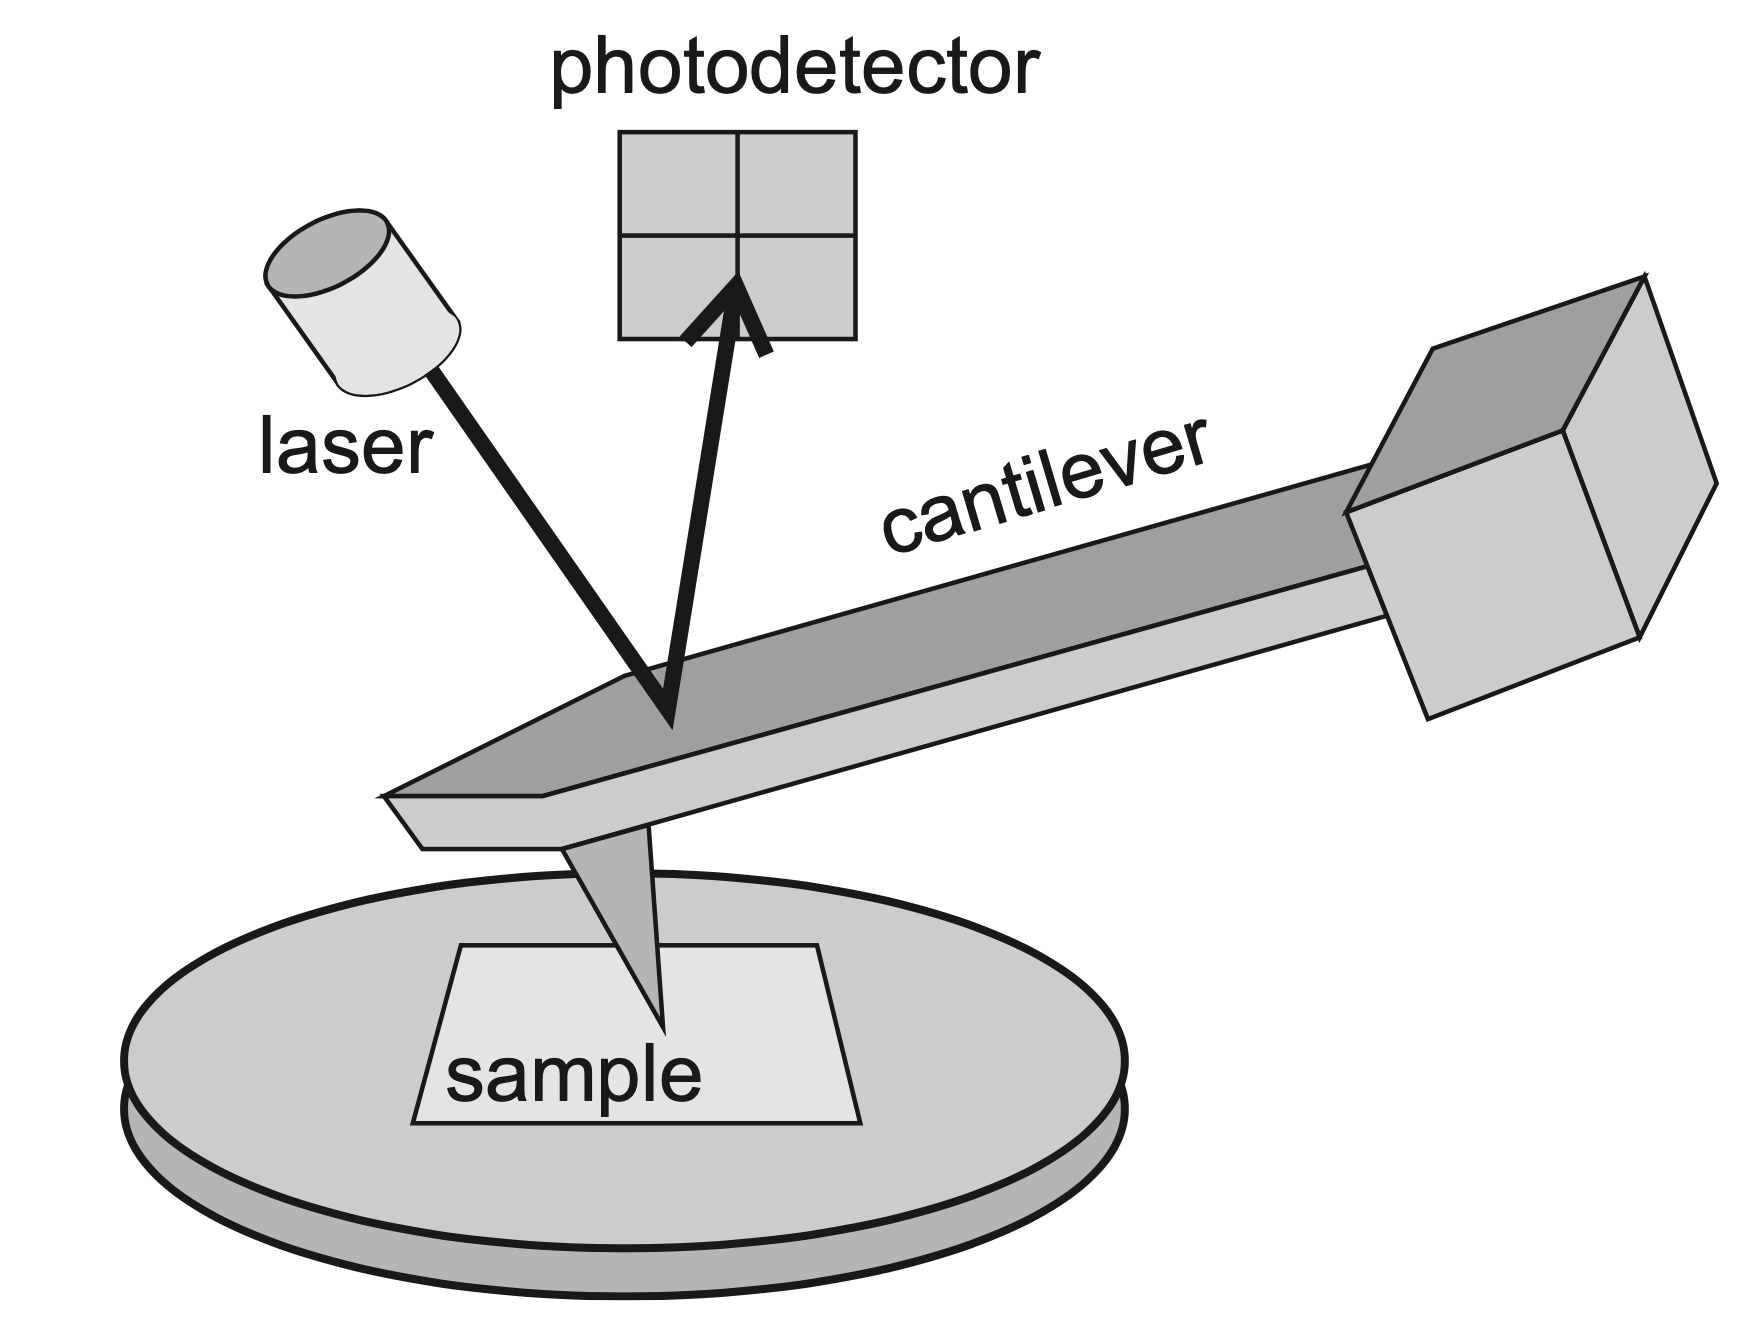
\includegraphics[width=0.6\linewidth]{figures/theory/AFM.png}
  \caption{\hl{Temporary} figure from \cite[p. 184]{gnecco_meyer_2015}}
  \label{fig:AFM}
\end{figure}


\acrshort{AFM} can also be used to drag a nanoflake accross the substrate as done by
Dienwiebel et al.\ \cite{DIENWIEBEL2005197}, where a graphene flake was attahced
to a \acrshort{FFM} tip and dragged accross graphite. Notice that this makes the normal
loading concentrated to a single point on the flake rather than achieving an evenly distributed load. 



\subsubsection{Surface Force Apparatus (SFA)}

\hl{I think this referes to having two interfaces sliding against each other with (optionally I think) lubrication between. This is often mirroed in MD simulations and often experimental results refer to this. So it might be worth saying a few words about, but I'm not sure yet.}



% Quartz Crystal Microbalance

% The trouble is that the coefficients of friction measured in nanotribological
% experiments and in macroscopic “tribotests” routinely differ by orders of
% magnitude. (\url{https://physicsworld.com/a/friction-at-the-nano-scale/})





% \subsection{Graphene friction}
% Theory of friction experiment involving graphene.


% Read Rare-gas islands and metal clusters \cite{Manini_2016} for theory of effects on surface area scaling

% Because of this frictional reduction, many studies indicate graphene as the
% thinnest solid-state lubricant and anti-wear coating [104–106]. (Current trends
% in the physics of nanoscale friction)


% Accurate FFM measurements on few-layer graphene systems show that friction
% decreases by increasing graphene thickness from a single layer up to 4-5 layers,
% and then it approaches graphite values [97, 99, 101, 107, 108]. (Current trends
% in the physics of nanoscale friction)


\subsection{Numerical procedures}



\section{Expected frictional properties of graphene}\label{sec:expected_prop}
In general we find three types of systems being studies for the frictional properties of graphene: 1) An \acrshort{AFM} type setup where the graphene, either resting on a substrate or in bulk graphite form, is probed by tip scanning across the surface. 2) Graphene sandwhiched between two substarte layers moving relative to each other using the graphene as a solid lubricant. 3) A graphene flake sliding on a substrate, either being dragged by an \acrshort{AFM} tip or by a similar applied force in numerical simulations. Only the latter matches our simulation setup, but we will consider results from all three categories due to a few amounts of studies following this approach. The relevant studies are listed as follows (maybe just tmp for my own sake).

\begin{enumerate}
  \item Setup % 1: AFM style (asperity related)
    \begin{enumerate}
      \item \cite{zhang_tuning_2019}: Exp., Straining sheet
      \item \cite{li_evolving_2016}: Num., Increasing layers,
      \item \cite{Yoon2015MolecularDS}: Num, silicon tip on graphene
      \item \cite{Paolicelli_2015}: Exp., graphene placed on SiO2 and Ni(111)substrates.
      \item \cite{Vazirisereshk_2019}: Exp., tip on graphene, MoS2 and Graphene/MoS2 heterostructure.
    \end{enumerate}
  \item Setup % 2: Sandwhich 
    \begin{enumerate}
      \item \cite{C2NR30691C}: Num., Corrugated nano-structured surfaces
      \item \cite{Wijn_2011}: Num., Rotational dynamics superlubricity
    \end{enumerate}
  \item Setup % 3: Flake on substrate
    \begin{enumerate}
      \item \cite{zhu_study_2018}: Num., graphene flake on gold substrate
      \item \cite{ma12091425}: Num., graphene on diamond, Orientation (Anisotropy)
      \item \cite{DIENWIEBEL2005197}: Exp., graphene on graphite, orientation and superlubricity
      \item \cite{feng_superlubric_2013}: Exp., graphene on graphite, orientation and superlubricity
      \item \cite{bonelli_atomistic_2009}: Num. (tight-binding), graphene on graphite.
      \item \cite{Reguzzoni_2012}, Num, graphene on graphite, varying layers (graphite thickness).
      \item \cite{liu_high-speed_2014}, Num, graphene on graphite, high speed 
    \end{enumerate}
\end{enumerate}



\begin{table}[H]
  \begin{center}
  \caption{...}
  \label{tab:friction_ref}
  \begin{tabular}{ |c|c|c|l|l|l| } \hline
    System & Type & Year & Researcher & materials & Info \\ \hline
  \multirow{5}{*}{1} & \multirow{3}{*}{Exp.} & 2019\cite{zhang_tuning_2019} & & Monolayer graphene  & Straining sheet \\ \cline{3-6} 
   & & 2015\cite{Paolicelli_2015} & & & graphene placed on SiO2 and Ni(111)substrates. \\ \cline{3-6} 
   & & 2019\cite{Vazirisereshk_2019} & & graphene, MoS2 and Graphene/MoS2 heterostructure & --- \\ \cline{2-6} 
   & \multirow{2}{*}{Num.}& 2016\cite{li_evolving_2016} & & Si tip on graphene (on a-Si substrate) & Increasing layers, \\ \cline{3-6} 
   & & 2015\cite{Yoon2015MolecularDS} & & silicon tip on graphene & --- \\ \cline{1-6} 
  \end{tabular}
  \end{center}
\end{table}





% Maybe open with a clarification on simulation /experimental setups.

Various simulation methods such as Molecular Dynamics (MD), Monte Carlo and ab initio calculations have been applied to investigate the diverse characteristics of graphene \cite{penkov_tribology_2014}. Especially \acrshort{MD} simulations for tribological properties have been used in the recent years.


% "Several studies have revealed the frictional behavior of graphene by varying different parameters such as the normal force, sliding velocity and graphene thickness."  \cite{penkov_tribology_2014}


% --- SIMULATIONS --- %
One of the earlist tribological simulations \cite{penkov_tribology_2014} of
graphene was Bonelli et al. \cite{bonelli_atomistic_2009} in 2009 using a
tight-binding method to simulate a graphene flake on an infinite graphene sheet.
Non rigid flake which could deform and rotate, but(?) the graphene flake was
fixed at a certain angle after applying normal force to reproduce \acrshort{AFM}
experiments. They found stick-slip behvaiour. The flake size and ``stacking
angle'' affected the frictional behaviour, such that a large area resulted in
experienced less friciton due the idea that the reactive atoms at the boundary
were dominant in increasing friction. The influence of the stacking angle was
attributed to the commensurability effect highlighted by the \acrshort{FK}
model. Similar bahviour in various structures such as carbon nano tubes CNT and
mice (what is mice) have previously been reported
\cite[41-42]{penkov_tribology_2014}. It has also been found that graphene (the
ideal nano-structure) exhibits superlubricity in cases of lattice mismatch.

% Thickness of graphene substrate
Reguzzoni et al. \cite[33]{penkov_tribology_2014} carried out a MD simulation of a graphene flake sliding sliding over a multi-layer (1-4) graphite substrate. They found that out-of-plane deformation of the graphene sheet (which one) increased with an increasing number of graphene layers. Meaning, that the vertical contatc stifness decreased with graphene thickness. Because frictional force and stick-slip motion were found to increase with decreasing stifness if was concluded that the single layer graphene were the best candidate for a solid nano-lubricant film. Moreover, the authors reported that the out-of-plane deformation nd the shear deformation induced by the stick-slip motion were the dominant factors incluencing friction.  


%CNT probing suspended graphene sheet
Smolyanitsky et al. \cite[34]{penkov_tribology_2014} performed a \acrshort{MD} simulation of a CNT probing a suspended graphene sheet. They found that for a positive normal force the friction generally increased with normal force, while for a negative normal force (as the tip pulled the suspended graphene due to adhesion) the friction increased for a decreasing normal force. This is in practive signs of a negative friction coefficient the negative range of normal load.  


% --- Experiments --- %

Maybe comment on the fact that most experiment use an FFM tip on a graphene sheet and not a graphene flake sliding on something else. 



% --- Lowering friction with strain --- %
% Tuning friction to a superlubric state via in-plane straining






% Articles to compare with
% https://www.mdpi.com/1996-1944/12/9/1425 Anisotropy of Graphene Nanoflake Diamond Interface Frictional Properties
% https://pubs.acs.org/doi/10.1021/nn305722d Superlubric Sliding of Graphene Nanoflakes on Graphene

% Also \cite{gao_frictional_2004} might be usefull to go through again

% Maybe rememeber to talk about the properties of asperity systems as the sheet creates asperities as it buckles. 

% Include "Molecular dynamics simulation of atomic-scale frictional behavior of corrugated nano-structured surfaces" somewhere.

The structural setup of our simulation is most reminiscent a graphene flake sliding on a substrate. This has been studied numerically in molecular dynamic simulations by Zhu and Li \cite[2018]{zhu_study_2018} for a graphene flake on a gold substrate and by Zhang et al.\ \cite{ma12091425}(2019) on a diamond substrate, and in a tight-binding simulation by Bonelli et al.\ \cite{bonelli_atomistic_2009}(2009) for graphene on graphite. Experimental studies of a graphene flake attatched to an AFM is done by Dienwiebel et al.\ \cite[2005]{DIENWIEBEL2005197} and Feng et al.\ \cite[2013]{feng_superlubric_2013} sliding on graphite, but these are mainly concerned with superlubricity due to flake oreientation commensurability. 

In our study we simmulate a graphene flake on a silicon substrate which deviates slightly from the above-mentioned references by having a different material combination. Additionally, the normal force is only applied to the ends of the sheet which might have an important effect. Obviously stretching and cutting the sheet will seperate our study dramatically from the references, but we aim to compare the frictional properties to the references before applying stretch or cuts. 
\\
\\
In the following we summarize the qualitative expections for the nanofriction behaviour for the unstretched and non-cut graphene sheet.
\subsubsection{Qualitatively}
\begin{enumerate}
  \item \textbf{Stick slip}: Generally we expect to observe periodic stick-slip motion with a period mathing the lattice constant(s) involved \cite{mo_friction_2009}. This was both present in the MD simulations \cite{zhu_study_2018}, \cite{ma12091425} and in the experiment by \cite{DIENWIEBEL2005197}. In AFM and SFA experiemnts, the stick-slip motion tend to transistion into smooth sliding when the speed exceeds $\sim \SI{1}{\mu/s}$ while in MD modelling the same transistion is observed in the $\sim \SI{1}{m/s}$ region \cite{Manini_2016}. Since we use a sliding speed of \SI{20}{m/s} we might transistion into smooth sliding. This 6 order of magnitude discrepancy has been largely discussed in connection to simplifying assumptions in MD simulations. Bonelli et al.\ \cite{bonelli_atomistic_2009} found that the stick-slip behaviour was present when the cantilever-tip-flake coupling was done with a relatively soft springs in contrast to hard springs which inhibited it.   

  \item \textbf{Static friction}: As highlighted in the FK model static friction
  will be sensitive to commensurability, which will additionally be affected by
  flake size. Reguzzoni and Righi \cite{PhysRevB.85.201412} have shown that the
  effective commensurability will increase drastically below a critical flake
  radius on the order of $10$ Å. Macroscopically we expect to see a logarithmic
  increase in static friction with contact time before sliding
  \cite{dieterich_1972}, and hence due to the short time-span of the static
  contact before dragging, it is not obvious to determine whether a significant
  static friction peak will be found. Also, the static friction best asserted by
  increasing the tangential sliding force slowly which is not the case in our
  simulation, especially considering that we are going to move the sheet rigidly
  (infinte spring constant) without any slack of a soft spring. Edge related
  origin of the pinning effects suggest that static friction can increase with
  sheet size up to a factor $A\propto A^{1/2}$, but this is also reported to be specific of the contact shape \cite{Manini_2016}.
  
  % Talk about size effects?

  % Concerning stick-slip friction, another problem is that, unlike simulations, real experiments contain mesoscale or macroscale component intrinsically involved in the mechanical instabilities of which stick-slip consists. Here the comforting observation is that stick-slip is nearly independent of speed, so that so long as a simulation is long enough to realize a sufficient number of slip events, the results may already be good enough [148]  \cite{Manini_2016}.


  % A serious aspect of stick-slip friction which MD simulation is unable to attack is ageing. The slip is a fast event, well described by MD, but sticking is a long waiting time, during which the frictional contact settles very slowly. The longer the sticking time, the larger the static friction force necessary to cause the slip. Typicall experiments show a logarithmic increase of static friction with time [150] \cite{Manini_2016}.
  
  % For monolayers sliding along atomically uniform substrates, however, there is
  % essentially no static friction. Indeed, the friction in these systems can be
  % up to 105 times less than that for macroscopic lubricants such as graphite.
  % This raises questions about the fundamental dissipation mechanisms that are at
  % work in systems at different scales.
  % (\url{https://physicsworld.com/a/friction-at-the-nano-scale/})

  \item \textbf{Oritentation (friction anisotropy)}: As predicted by the FK model and confirmed both numerically \cite{zhu_study_2018}, \cite{ma12091425} and experimentally \cite{DIENWIEBEL2005197}, \cite{feng_superlubric_2013} we expect a dependence of friction force on orientation due to changing commensurability. Zhu and Li \cite{zhu_study_2018} (gold substrate) reported the highest friction when sliding along the armchair direction, while Zhang et al.\ \cite{ma12091425} (diamond substrate) found the zigzag-direction to give the highest friction force (also the most evident stick-slip behvaiour in this direction). 
\end{enumerate}


By consulting with the most related numerical and experimental studies, while also considering the theoretical gap between smooth atomic contact and asperity theory, we have summarized an evaluation of the most important quantative trends expected from our numerical results in \cref{var_dep}. 


\begin{table}[H]
  \begin{center}
  \caption{Quantitative nano friction dependence on various variables. \hl{work in progress.}}
  \label{tab:var_dep}
  \begin{tabular}{ | c | C{3cm}| m{5cm}| m{5cm}|} \hline
  \textbf{Variable} & \textbf{Dependency} & \textbf{Numerical studies} & \textbf{Experimental} \\ \hline 
  Normal force $F_N$ 
  & {\begin{align*}
    F_{\text{fric}} &\propto F_N^{\alpha} \\
    \alpha &\le 1
  \end{align*}} 
  & Zhang et al.\ \cite{ma12091425} finds a seemingly linear relationship $F_{\text{fric}} \propto F_N$ while Bonelli et al.\ \cite{bonelli_atomistic_2009} reports a sublinear relationship. The latter corresponds with that of nanosasperity simulations where Mo et al.\ \cite{mo_friction_2009}, using an amorphous carbon tip on a diamond sample, also found a sublinear relationship when including adhesion and linear without adhesion.
  & Experimentally rather different trends have been observed, although the majority agree on increasing friction with increasing load \cite[p. 200]{gnecco_meyer_2015}. For the graphebne flake Dienwiebel et al.\ \cite{DIENWIEBEL2005197} found a seemingly non-dependent relationship while Feng et al.\ \cite{feng_superlubric_2013} did not report on this. FFM analog to the single asperity setup have yielded both linear relationship \cite{gao_frictional_2004} (silicon tip on gold) while Schwarz et al.\ \cite{PhysRevB.56.6987} found that FFM with well-defined spherical tips mathed with theoretical results (DMT, elastic spheres pressed together \cite[p. 200]{gnecco_meyer_2015}), yielding a power law $F_{\text{fric}} = F_N^{2/3}$. 
  \\ \hline
  Velocity $v$ & 
  {\begin{align*}
    F_{\text{fric}} &\propto \ln{v} \ (\text{exp.})\\
    &\text{or} \\
    F_{\text{fric}} &\propto v \ (\text{num.})\\
  \end{align*}}
  % $F_{\text{fric}} \propto \ln{v}$ 
  &  Studies of gold clusters on graphite suggest that friction is viscous, i.e. proportional to velocity \cite{Manini_2016}.

  & Logaritmic velocity dependence of friction has been measured for nanotip friction \cite[p. 201]{gnecco_meyer_2015} associated to thermal activation and possibly the time availble to form bond between the tip and the substrate. At higher velocities thermally activated processes are less important and friction becomes independent of velocity. This has been observed for Si tips and diamond, graphite and amorphous carbon surfaces with scan velocities above \SI{1}{\mu/s}.
  \\ \hline
  Temperature $T$
  & Either increase (MD) or decrease as $F_{\text{fric}} \propto \exp{(1/T)}$  (experimental)
  &  Zhang et al.\ \cite{ma12091425} found simply that friction increased with temperature. The \cite{Manini_2016} gold cluster on graphite study (\hl{get reference}) found that the temperature dependence was dependend on velocity regime. Low speed (diffusive) friction decreases upon heating while high speed (ballistic) friction rises with temperature. 
  & Zhao et al.\ \cite{zhao_thermally_2007} found $F_{\text{fric}} \propto \exp({1/T})$.
  \\ \hline
  Real contact area $A$ 
  & $F_{\text{fric}} \propto A$ 
  & Mo et al.\ \cite{mo_friction_2009} found that $F_{\text{fric}} \propto A$ where $A$ is the real contact area defined by atoms within chemical range. This is not studied for the case of a nanoflake where the contact area is presumingly rather constant.
  & \\ \hline
  \end{tabular}
  \end{center}
\end{table}


% As anticipated in Sec. 4.2, MD simulation is an ideal tool for the study of friction in fast-sliding of nanosized systems. Using gold clusters on graphite as test system, simulation has explored high-speed friction, and especially differences and similarities from low speed, examining the slowing down of a ballistically kicked cluster. Both kinetic frictions are similarly viscous – proportional to velocity. However, they show just the opposite thermal dependence. Whereas low speed (diffusive) friction decreases upon heating, when diffusion increases, the high speed (ballistic) friction rises with temperature, when thermal fluctuations of the contact increase [200]. \cite{Manini_2016}

% \begin{table}[H]
%   \begin{center}
%   \caption{Quantitative nano friction dependence on various variables.}
%   \label{tab:var_dep}
%   \begin{tabular}{ | c | m{3cm}| m{5cm}| m{5cm}|} \hline
%   \textbf{Variable} & \textbf{Dependency} & \textbf{Numerical studies} & \textbf{Experimental} \\ \hline 
%   Normal force $F_N$ 
%   &  $F_f$ increasing $F_N$
%   & MD simulations of amorphous carbon asperity on diamond substrate suggest a linear relatioship to $F_f\propto F_N$ for nonadhesive contact and sublinear with van der waals adhesive forces \cite{mo_friction_2009}. Graphene flake?
%   & The general trend observed in AFM nanoscale friction is that friction force increase with normal load \cite[p.200]{gnecco_meyer_2015}. Various trends have been observed from linear to power trends. 
%   \\ \hline
%   Velocity $v$& $F_f \propto \ln{v}$ & & \\ \hline
%   Temperature $T$& $F_f \propto 1/T$ & & \\ \hline
%   Real contact area $A$ & $F_f \propto A$ & & \\ \hline
%   \end{tabular}
%   \end{center}
% \end{table}




% the stick-slip motion was more evident when changing the sliding direction from armchair to zigzag direction \cite{ma12091425}
  
%   \subsubsection{Variable dependence}

%   \begin{enumerate}
%   \item Normal force: The general trend observed in AFM nanoscale friction is that friction force increase with normal load \cite{gnecco_meyer_2015}. 
%   \item Velocity: Smooth kinetic friction generally increase with speed (velocity strengthening) \cite{Manini_2016}. E. Gnecco et al.\ \cite{PhysRevLett.84.1172} showed a logaritmic increase in mean friction with velocity (the tip of a friction force microscope and NaCl(100) at low velocity ($10^-9$ - $10^-6$ m/s)).  If the scan velocity increases thermally activated processes becomes less important and beyond a critical value the friction forces becomes independent of velocity \cite[p. 202]{gnecco_meyer_2015}
%   \item Temperature: A decrease in friction as $1/T$ was observed by Zhao et al.\ in a series of AFM measurements on graphite in a wide temperature range (140-750 K) \cite[source 351]{gnecco_meyer_2015}
%   % Zhao et al.\ (2007) observed that friction on graphite decreases as 1/T over a wide temperature range (140–750 K), supporting the hypothesis of thermal activation of the stick–slip process. However, it was only recently that group of Schirmeisen reported atomic-scale FFM mea- surements in UHV at different temperatures (Jan- sen et al.\ 2010). When silicon, SiC, ionic crystals and graphite surfaces were cooled down from room temperature to cryogenic conditions, a good agreement with the thermally activated PT model was found down to a peak or a plateau, appearing between 50 and 200 K. Below these values, the friction was found to decrease with temperature, which the authors attributed to the competition between thermally activated rupture and formation of chemical bonds (Barel et al.\ 2010). \cite{BHUSHAN20051507}
%   \item Ruan and Bhushan (1994) (source) found in an AFM study on graphite that the friction coefficient was around $\sim 0.01 - 0.03$
%   % Ruan and Bhushan (1994) used an AFM to investigate the effect of surface roughness on the tribological characteristics of graphite using a Si3N4 tip. It was found that friction coefficient varied with respect to roughness of the substrate. The friction coefficient was below 0.01 and 0.03 for RMS roughness of about 10 nm and 140 nm, respectively. This outcome was attributed to the loss of orientation of the substrate with increasing roughness.33 \cite{kim_nano-scale_2009}
%   \item Contact area
% \end{enumerate}






% \begin{enumerate}
%   \item Smooth kinetic friction generally increase with speed  \cite{Manini_2016}. so-called velocity strengthening.  Logaritmic with speed % Gnecco E, Bennewitz R, Gyalog T, Loppacher C, Bam- merlin M, Meyer E, Güntherodt H-J (2000) Velocity dependence of atomic friction. Phys Rev Lett 84:1172–1175. Maybe crosscheck with macroscale to ensure that this is valid for higher velocities. 
 
%   \item Occurrence of stick slip (also in MD) \cite{kim_nano-scale_2009} (p. 146)
% \end{enumerate}

% Thus, it is commonly expected that the
% friction of a dry nanocontact should classically decrease with increasing
% temperature provided no other surface or material parameters are altered by
% the temperature changes [77, 80–83]. (Current trends in the physics of
% nanoscale friction)

% Thus far we have used thermal activation to explain the velocity dependence of friction. The same mechanism also predicts that friction should change with temperature. \cite{BHUSHAN20051507}








% Look for source on affect on friction when stretching. Since we control the area through that there might be a stretch effect that is even stronger. 





% 

% Hint for explaining increase with stretch: Both micro-tribotester and AFM were used to investigate the micro/nano frictional behavior. It was reported that contact angle between the groove and the pin affected the frictional characteristics significantly. High contact angle led to a sudden increase in the frictional force due to interlocking mechanism. \cite{kim_nano-scale_2009}
% These works suggest that frictional behavior at micro/nano scale is very much dependent on the surface structure and topography. Furthermore, the contact geometry between the tip and the surface such as area and orientation of the contacting angle affect the frictional force significantly. \cite{kim_nano-scale_2009}



% Should period macth the lattice spacing as described in \cite{kim_nano-scale_2009}[p. 144]



% Maybe talk about the slip line as shown in \cref{fig:slip_line}


% \begin{figure}[H]
%   \centering
%   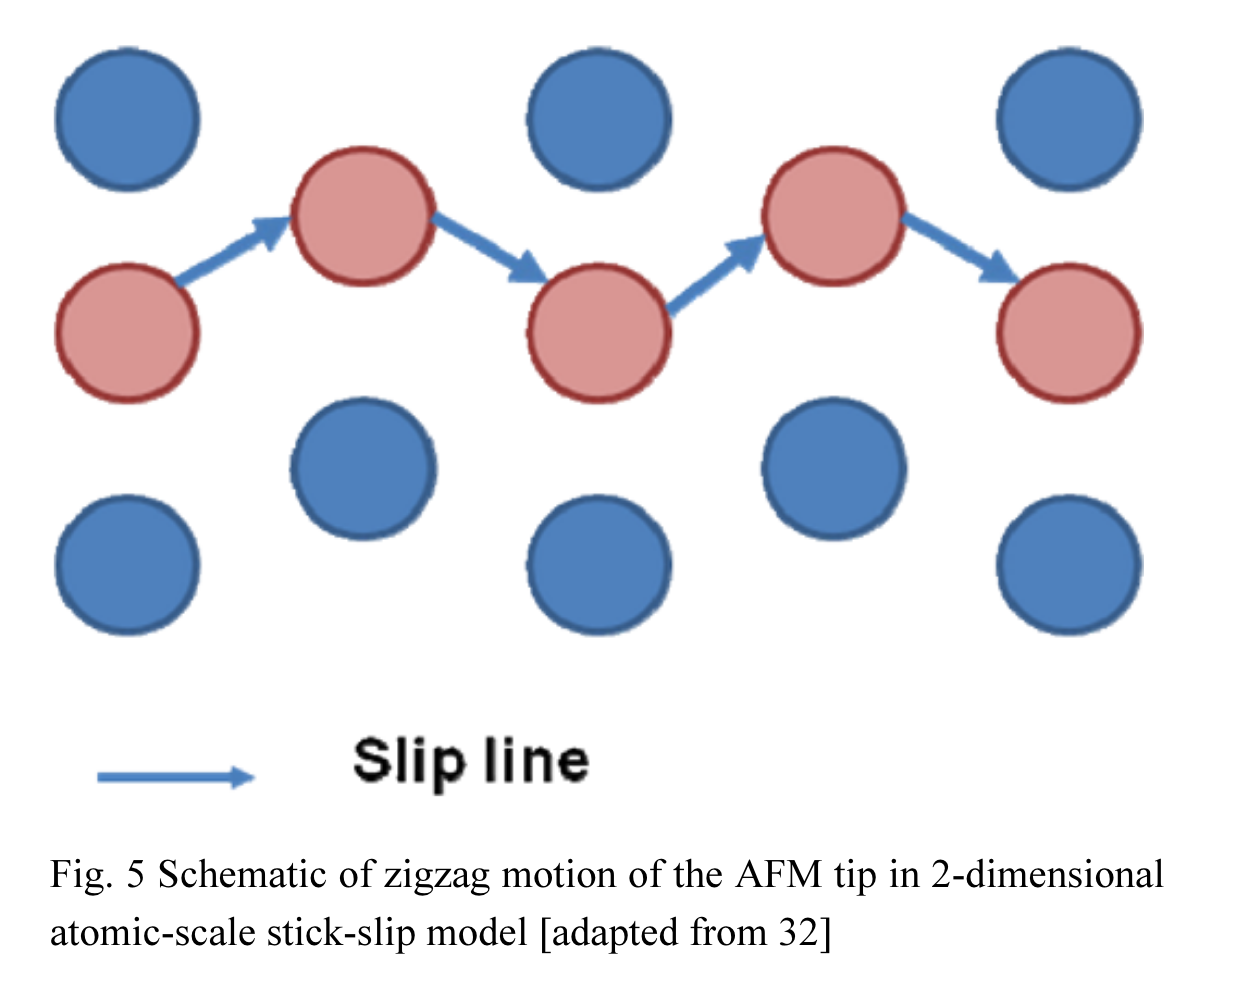
\includegraphics[width=0.5\linewidth]{figures/theory/slip_line.png}
%   \caption{\hl{Temporary} figure from \cite{kim_nano-scale_2009}[p. 144]}
%   \label{fig:slip_line}
% \end{figure}

% \begin{enumerate}
%   \item Friction should decrease by increasing temperature.
%   \item We expect stick slip motion
%   \item What about dependence on normal force?
%   \item Dependence on contact area?
%   \item Dependense on speed? 
% \end{enumerate}

% \begin{itemize}
%   \item Different friction models on macro-and microscopic scale
% \end{itemize}


% Smooth kinetic friction generally increases with speed (velocity strengthening), but sometimes decreases with increasing speed in certain intervals \cite{Manini_2016}.

% the smallest force needed to set a slider in motion – is also dependent on the simulation time (a longer wait may lead to depinning when a short wait might not), and generally dependent on system size, often increasing with sub-linear scaling with the slider’s contact area. To address this kind of behavior in MD simulations, it is often necessary to resort to scaling arguments in order to extrapolate the large-area static friction from small-size MD simulations [131, 140] \cite{Manini_2016}.


% Section 15.3. As shown in Section 15.1, the maximum value of the static friction and the slope of the turning points of the F(x) curves can be used to determine the corrugation U0 of the tip–surface interaction potential and the effective lat- eral stiffness k of the system. From Fig. 18.1(b) we estimate U0 ≈ 0.22 eV and k ≈1N/m. \cite{gnecco_meyer_2015} p. 197






% Concerning stick-slip friction, another problem is that, unlike simulations, real experiments contain mesoscale or macroscale component intrinsically involved in the mechanical instabilities of which stick-slip consists. Here the comforting observation is that stick-slip is nearly independent of speed, so that so long as a simulation is long enough to realize a sufficient number of slip events, the results may already be good enough [148]  \cite{Manini_2016}.


% A serious aspect of stick-slip friction which MD simulation is unable to attack is ageing. The slip is a fast event, well described by MD, but sticking is a long waiting time, during which the frictional contact settles very slowly. The longer the sticking time, the larger the static friction force necessary to cause the slip. Typicall experiments show a logarithmic increase of static friction with time [150] \cite{Manini_2016}.

% Rate and state friction approaches, widely used in geophysics [151], describe phenomenologically frictional ageing, but a quantitative microscopic description is still lacking. Mechanisms invoked to account for contact ageing include chemical strengthening at the interface in nanoscale systems [152], and plastic creep phenomena in macroscopic systems [153]. \cite{Manini_2016}.


% See ``Selected Results of MD Simulations'' in \cite{Manini_2016} p. 24.

% \section{Real life experimental procedures}
% From Introduction to Tribology, Second Edition, p. 526: \par The surface force
% apparatus (SFA), the scanning tunneling microscopes (STM), and atomic force and
% friction force microscopes (AFM and FFM) are widely used in nanotribological and
% nanomechanics studies.



\section{Research questions}

% Formulate the research questions guiding the reading of the thesis moving on. 